% ==============================================================================
% ISCAE PFE — Rapport de fin d'études
% Sujet : WebCyber — Conception, déploiement et analyse de sécurité
%         d'une application web sur AWS via la conteneurisation Docker
%
% Compilation : XeLaTeX ou LuaLaTeX (Times New Roman via fontspec)
%               sur Overleaf, choisir XeLaTeX dans les paramètres du projet.
% ==============================================================================
\documentclass[12pt,a4paper]{report}

% ---------- Polices et typographie ----------
\usepackage{fontspec}
\setmainfont{Times New Roman}
\usepackage{microtype}
\usepackage{setspace}
\onehalfspacing

% ---------- Langue ----------
\usepackage[french]{babel}

% ---------- Mise en page et graphiques ----------
\usepackage{geometry}
\geometry{left=2.2cm,right=2.2cm,top=2.2cm,bottom=2.2cm}
\usepackage{graphicx}
\usepackage{float}
\usepackage{xcolor}
\usepackage{tikz}
\usetikzlibrary{positioning}
\usepackage{standalone}      % permet \input des diagrammes standalone

\usepackage{parskip}
\setlength{\parindent}{0pt}
\setlength{\emergencystretch}{3em}

% ---------- Citations ----------
\usepackage{cite}

% ---------- Tableaux ----------
\usepackage{array}
\usepackage{booktabs}
\usepackage{longtable}
\usepackage{ragged2e}
\newcolumntype{P}[1]{>{\RaggedRight\arraybackslash}m{#1}}
\newcolumntype{C}[1]{>{\centering\arraybackslash}m{#1}}
\newcolumntype{R}[1]{>{\RaggedLeft\arraybackslash}m{#1}}

% ---------- Code source ----------
\usepackage{listings}
\definecolor{codebg}{RGB}{248,249,250}
\definecolor{codecomment}{RGB}{106,153,85}
\definecolor{codekeyword}{RGB}{0,102,153}
\definecolor{codestring}{RGB}{163,21,21}
\lstset{
  basicstyle=\ttfamily\footnotesize,
  backgroundcolor=\color{codebg},
  commentstyle=\color{codecomment}\itshape,
  keywordstyle=\color{codekeyword}\bfseries,
  stringstyle=\color{codestring},
  numbers=left,
  numberstyle=\tiny\color{gray},
  numbersep=6pt,
  frame=single,
  rulecolor=\color{lightgray},
  framesep=4pt,
  breaklines=true,
  showstringspaces=false,
  tabsize=2,
  captionpos=b,
  literate={é}{{\'e}}1 {è}{{\`e}}1 {ê}{{\^e}}1 {à}{{\`a}}1
           {ç}{{\c{c}}}1 {ô}{{\^o}}1 {î}{{\^\i}}1 {ï}{{\"\i}}1
           {ù}{{\`u}}1 {É}{{\'E}}1 {È}{{\`E}}1 {À}{{\`A}}1
}

% ---------- Titres ----------
\usepackage{titlesec}

% ---------- Couleurs ----------
\definecolor{iscaeblue}{RGB}{0,102,153}
\definecolor{lightgray}{RGB}{245,245,245}

% ==============================================================================
% MÉTADONNÉES — à modifier pour chaque projet
% ==============================================================================
\newcommand{\Institute}{Institut Supérieur de Comptabilité et d'Administration des Entreprises}
\newcommand{\Location}{Nouakchott --- Mauritanie}
\newcommand{\LogoFile}{logo-iscae.png}

% Étudiant (un seul auteur sur ce projet)
\newcommand{\studentA}{Mohamed Salem KHYARHOUM --- I19xxx}

\newcommand{\supervisor}{Nom de l'encadreur}
\newcommand{\company}{ISCAE Nouakchott}
\newcommand{\academicYear}{2025--2026}
\newcommand{\projectTitle}{Conception, déploiement et analyse de sécurité d'une application web hébergée sur AWS via la conteneurisation Docker}
\newcommand{\projectType}{PROJET DE FIN D'ÉTUDES}
\newcommand{\degree}{LICENCE en Développement Informatique}

% ==============================================================================
% Hyperliens
\usepackage{hyperref}
\hypersetup{
  colorlinks=true,
  linkcolor=black,
  citecolor=blue,
  urlcolor=blue,
  pdftitle={\projectTitle},
  pdfauthor={\studentA}
}

% ==============================================================================
% Redéfinition des chapitres (page de garde par chapitre)
\makeatletter
\let\OldChapter\chapter

\newcommand{\MyChapterPage}[2]{%
  \clearpage
  \thispagestyle{empty}
  \begin{center}
    \vspace*{0.30\textheight}
    {\Huge\bfseries Chapitre\ \ #1\\[1.5ex] #2}
  \end{center}
  \clearpage
}

\def\MyChapter#1{%
  \refstepcounter{chapter}%
  \phantomsection
  \addcontentsline{toc}{chapter}{\protect\numberline{\thechapter}#1}%
  \markboth{#1}{#1}%
  \MyChapterPage{\thechapter}{#1}%
}

\def\MyChapterStar#1{%
  \clearpage
  \thispagestyle{plain}%
  \OldChapter*{#1}%
  \addcontentsline{toc}{chapter}{#1}%
}

\renewcommand{\chapter}{\@ifstar{\MyChapterStar}{\MyChapter}}
\makeatother

% ==============================================================================
% DÉBUT DU DOCUMENT
% ==============================================================================
\begin{document}

\pagenumbering{roman}
\pagestyle{plain}

% ---------------- Page de garde ----------------
\begin{titlepage}
\thispagestyle{empty}

\begin{tikzpicture}[remember picture,overlay]
\draw[line width=2pt,color=iscaeblue]
    ([xshift=1cm,yshift=-1cm]current page.north west)
    rectangle
    ([xshift=-1cm,yshift=1cm]current page.south east);
\draw[line width=0.8pt,color=iscaeblue]
    ([xshift=1.2cm,yshift=-1.2cm]current page.north west)
    rectangle
    ([xshift=-1.2cm,yshift=1.2cm]current page.south east);
\end{tikzpicture}

\begin{center}

{\large \textbf{\Institute}}\\[0.2cm]
{\itshape \Location}

\vspace{0.8cm}

\IfFileExists{\LogoFile}{\includegraphics[width=3cm]{\LogoFile}}{%
  \fbox{\parbox[c][3cm][c]{3cm}{\centering\itshape\small Logo ISCAE\\(à insérer)}}%
}

\vspace{0.5cm}
\hrule
\vspace{0.5cm}

{\Large \bfseries\colorbox{yellow}{\projectType}}

\vspace{0.5cm}

Pour l'obtention de :\\[0.2cm]
{\large \bfseries\colorbox{yellow}{\degree}}

\vspace{0.8cm}

\textbf{Thème :}

\vspace{0.4cm}

\fbox{\parbox{0.98\linewidth}{\centering\fontsize{11}{12}\selectfont\textbf{\projectTitle}}}

\vspace{1cm}

\begin{flushleft}
\textit{Élaboré par :}
\end{flushleft}

\begin{center}
\colorbox{yellow}{\studentA}\\[0.2cm]
\end{center}

\vspace{0.8cm}

\begin{flushleft}
\textit{Encadré par :}
\end{flushleft}

\begin{center}
\colorbox{yellow}{\supervisor}
\end{center}

\vfill

{\itshape Année Universitaire : \academicYear}

\end{center}
\end{titlepage}

% ---------------- Pages liminaires ----------------
\chapter*{Dédicaces}
\thispagestyle{empty}

\vspace{2cm}

\begin{center}
\itshape

\textit{À mes parents,}\\[0.5em]
qui m'ont soutenu sans relâche tout au long de mes études et qui n'ont
jamais cessé de croire en moi.\\[1.5em]

\textit{À mes frères et sœurs,}\\[0.5em]
pour leurs encouragements constants et leur présence chaleureuse.\\[1.5em]

\textit{À mes enseignants,}\\[0.5em]
qui m'ont transmis le goût du savoir et la rigueur du travail bien fait.\\[1.5em]

\textit{À mes camarades de promotion,}\\[0.5em]
avec qui j'ai partagé tant d'heures de travail, de doutes et de réussites.\\[1.5em]

\textit{À tous ceux qui, de près ou de loin,}\\[0.5em]
ont contribué à la concrétisation de ce projet,\\
je dédie ce modeste travail.

\vfill

\textsc{Mohamed Salem}
\end{center}

\chapter*{Remerciements}
\thispagestyle{empty}

Au terme de ce projet de fin d'études, je tiens à exprimer ma profonde
reconnaissance à toutes les personnes qui, par leur soutien, leurs conseils
ou leur présence, ont contribué à l'aboutissement de ce travail.

\vspace{0.6em}

Je remercie tout d'abord \textbf{Allah le Tout-Puissant} de m'avoir donné
la santé, la patience et la volonté nécessaires pour mener à bien ce projet.

\vspace{0.6em}

Mes plus sincères remerciements s'adressent à mon encadrant,
\textbf{\supervisor}, pour sa disponibilité, ses conseils éclairés et son
suivi rigoureux tout au long de la réalisation de ce projet. Ses
remarques pertinentes m'ont permis d'orienter mon travail dans la bonne
direction et d'en améliorer la qualité.

\vspace{0.6em}

Je tiens également à remercier l'ensemble du corps enseignant de
\textbf{l'\Institute} pour la qualité de la formation reçue durant mes
années d'études, ainsi que pour l'environnement académique stimulant
qu'ils ont su créer.

\vspace{0.6em}

Mes remerciements vont aussi aux \textbf{membres du jury} qui ont accepté
d'évaluer ce travail. Leurs critiques constructives constitueront une
précieuse contribution à mon développement professionnel futur.

\vspace{0.6em}

Enfin, j'adresse une pensée toute particulière à ma \textbf{famille} et à
mes \textbf{amis} pour leur soutien indéfectible, leur patience et leurs
encouragements, qui m'ont permis de surmonter les moments difficiles et
d'aller jusqu'au bout de cette aventure.

\vspace{1em}

À toutes et à tous, \textbf{merci}.

\chapter*{Résumé}
\thispagestyle{empty}

Ce projet de fin d'études porte sur la conception, le développement,
le déploiement et l'analyse de sécurité d'une application web de prise
de notes personnelle, baptisée \textbf{WebCyber}. L'application repose
sur le \emph{framework} Python \textbf{Flask} pour la couche métier,
sur \textbf{PostgreSQL} pour la persistance des données, et sur
\textbf{Nginx} comme proxy inverse assurant la terminaison TLS.
L'ensemble est \textbf{conteneurisé} avec Docker et orchestré via Docker
Compose, puis \textbf{déployé sur AWS} (instance EC2 \texttt{t2.micro}
sous Ubuntu Server 22.04 LTS), avec une résolution de nom de domaine
gérée par \textbf{Route\,53} et un certificat HTTPS automatique fourni
par \textbf{Let's Encrypt}.

\vspace{0.4em}

Une attention particulière a été portée à la sécurité, organisée
en \textbf{six couches} : pare-feu réseau (\emph{Security Group} AWS),
durcissement du système, isolation Docker, configuration TLS et
en-têtes de sécurité Nginx, contrôles applicatifs (authentification,
hachage \texttt{PBKDF2-SHA256}, protection CSRF, validation des
entrées, isolation des données par utilisateur) et sécurité de la
base de données. La solution déployée a ensuite été soumise à une
campagne d'évaluation à l'aide de \textbf{Nmap}, \textbf{Nikto} et
\textbf{testssl.sh}, dont les résultats sont analysés et discutés.

\vspace{0.4em}

\textbf{Mots-clés :} application web, sécurité, cybersécurité, AWS,
EC2, Docker, conteneurs, Nginx, Flask, PostgreSQL, HTTPS, TLS,
Let's Encrypt, Nmap, Nikto, défense en profondeur, DevOps.

\vspace{1.5em}

\begin{center}
\noindent\rule{0.6\linewidth}{0.4pt}
\end{center}

\vspace{0.8em}

\section*{Abstract}

This end-of-studies project covers the design, development, deployment
and security assessment of a personal note-taking web application named
\textbf{WebCyber}. The application is built on the Python
\textbf{Flask} framework for business logic, \textbf{PostgreSQL} for
data persistence, and \textbf{Nginx} as a reverse proxy handling TLS
termination. The whole stack is \textbf{containerised} with Docker and
orchestrated through Docker Compose, then \textbf{deployed on AWS}
(EC2 \texttt{t2.micro} instance running Ubuntu Server 22.04 LTS), with
DNS resolution provided by \textbf{Route\,53} and HTTPS certificates
automatically issued by \textbf{Let's Encrypt}.

\vspace{0.4em}

Security has been treated as a first-class concern and structured into
\textbf{six layers}: AWS Security Group network firewall, host
hardening, Docker isolation, Nginx TLS and security headers,
application-level controls (authentication, \texttt{PBKDF2-SHA256}
password hashing, CSRF protection, input validation, per-user data
isolation) and database security. The deployed solution was then
assessed using \textbf{Nmap}, \textbf{Nikto} and \textbf{testssl.sh},
and the results are analysed and discussed.

\vspace{0.4em}

\textbf{Keywords:} web application, security, cybersecurity, AWS, EC2,
Docker, containers, Nginx, Flask, PostgreSQL, HTTPS, TLS, Let's Encrypt,
Nmap, Nikto, defense-in-depth, DevOps.


% ---------------- Tables ----------------
\renewcommand{\contentsname}{Table des matières}
\tableofcontents
\clearpage

\renewcommand{\listfigurename}{Liste des figures}
\listoffigures
\clearpage

\renewcommand{\listtablename}{Liste des tableaux}
\listoftables
\clearpage

% ---------------- Acronymes ----------------
\chapter*{Liste des acronymes}
\addcontentsline{toc}{chapter}{Liste des acronymes}

\begin{longtable}{p{3cm} p{12cm}}
\toprule
\textbf{Acronyme} & \textbf{Signification} \\
\midrule
\endhead

ACME & \textit{Automatic Certificate Management Environment} (protocole Let's Encrypt) \\
AMI  & \textit{Amazon Machine Image} \\
API  & \textit{Application Programming Interface} \\
AWS  & \textit{Amazon Web Services} \\
CI/CD & \textit{Continuous Integration / Continuous Deployment} \\
CIDR & \textit{Classless Inter-Domain Routing} \\
CRUD & \textit{Create, Read, Update, Delete} \\
CSP  & \textit{Content Security Policy} \\
CSRF & \textit{Cross-Site Request Forgery} \\
DNS  & \textit{Domain Name System} \\
EBS  & \textit{Elastic Block Store} \\
EC2  & \textit{Elastic Compute Cloud} \\
EIP  & \textit{Elastic IP Address} \\
GHA  & \textit{GitHub Actions} \\
GHCR & \textit{GitHub Container Registry} \\
HSTS & \textit{HTTP Strict Transport Security} \\
HTTP & \textit{Hypertext Transfer Protocol} \\
HTTPS & \textit{HTTP Secure} \\
IaaS & \textit{Infrastructure as a Service} \\
IaC  & \textit{Infrastructure as Code} \\
IGW  & \textit{Internet Gateway} \\
IDOR & \textit{Insecure Direct Object Reference} \\
IMDSv2 & \textit{Instance Metadata Service version 2} \\
IP   & \textit{Internet Protocol} \\
LTS  & \textit{Long-Term Support} \\
MVC  & \textit{Modèle-Vue-Contrôleur} \\
NIST & \textit{National Institute of Standards and Technology} \\
ORM  & \textit{Object-Relational Mapping} \\
OWASP & \textit{Open Web Application Security Project} \\
PaaS & \textit{Platform as a Service} \\
PBKDF2 & \textit{Password-Based Key Derivation Function 2} \\
PFE  & Projet de Fin d'Études \\
SaaS & \textit{Software as a Service} \\
SAST & \textit{Static Application Security Testing} \\
SG   & \textit{Security Group} \\
SQL  & \textit{Structured Query Language} \\
SSH  & \textit{Secure Shell} \\
SSL  & \textit{Secure Sockets Layer} \\
TCP  & \textit{Transmission Control Protocol} \\
TLD  & \textit{Top-Level Domain} \\
TLS  & \textit{Transport Layer Security} \\
URL  & \textit{Uniform Resource Locator} \\
UML  & \textit{Unified Modeling Language} \\
VPC  & \textit{Virtual Private Cloud} \\
WSGI & \textit{Web Server Gateway Interface} \\
XSS  & \textit{Cross-Site Scripting} \\
\bottomrule
\end{longtable}


% ---------------- Corps du rapport ----------------
\clearpage
\pagenumbering{arabic}
\setcounter{page}{1}

\chapter*{Introduction générale}
\markboth{Introduction générale}{Introduction générale}

\section*{Contexte}

À l'ère de la transformation numérique, la majorité des services
quotidiens — communication, gestion documentaire, commerce,
administration — repose sur des applications web hébergées dans le
\emph{cloud}. Cette omniprésence du Web s'est accompagnée d'une
explosion des incidents de sécurité : selon le rapport
\textit{Verizon Data Breach Investigations Report 2023}, plus de 80\,\%
des compromissions enregistrées exploitent des vulnérabilités
applicatives ou des erreurs de configuration. Concevoir une application
web ne se résume donc plus à coder un service fonctionnel : il faut
également maîtriser son hébergement, son réseau, son cycle de
déploiement et sa surface d'attaque.

Le mouvement \emph{DevOps} et l'adoption généralisée des \textbf{conteneurs}
ont profondément changé la manière de construire et de livrer ces
applications. Docker offre une portabilité quasi parfaite entre les
environnements de développement et de production, tandis que les
fournisseurs de \emph{cloud} comme \textbf{Amazon Web Services} (AWS)
permettent de provisionner en quelques minutes des infrastructures
auparavant réservées aux grands centres de données. La maîtrise de
ces outils est désormais une compétence attendue de tout développeur
ou administrateur système.

\section*{Problématique}

Si les briques technologiques sont accessibles, leur \emph{intégration
sécurisée} reste un exercice difficile : combien de bases de données
exposées sur Internet, combien de certificats expirés, combien
d'applications vulnérables aux injections SQL ou au \emph{cross-site
scripting} ?

La problématique de ce projet peut être formulée ainsi :

\begin{quote}
\itshape Comment concevoir, développer et déployer une application
web fonctionnelle dans le \emph{cloud}, en appliquant de manière
explicite et vérifiable les bonnes pratiques de cybersécurité, depuis
la couche réseau jusqu'au code applicatif ?
\end{quote}

\section*{Objectifs}

Le projet \textbf{WebCyber} apporte une réponse pédagogique et
pragmatique à cette problématique en poursuivant les objectifs
suivants :

\begin{enumerate}
  \item Concevoir une application web simple mais réaliste : une
        application personnelle de prise de notes (CRUD complet,
        authentification, isolation des données par utilisateur).
  \item Conteneuriser l'ensemble des composants (Nginx, application
        Flask, base PostgreSQL) avec Docker et Docker Compose.
  \item Déployer la solution sur une infrastructure AWS minimaliste
        mais représentative (EC2, Elastic IP, Security Group, Route\,53).
  \item Mettre en œuvre une chaîne de sécurité \textbf{en profondeur}
        couvrant le réseau, le système, les conteneurs, le proxy, le
        code applicatif et la base de données.
  \item Activer HTTPS via un certificat Let's Encrypt, avec
        renouvellement automatisé.
  \item Évaluer la posture de sécurité du déploiement à l'aide
        d'outils standard (Nmap, Nikto, testssl.sh) et discuter les
        résultats.
  \item Rédiger une documentation technique exploitable permettant à
        un autre étudiant ou ingénieur de reproduire la solution.
\end{enumerate}

\section*{Plan du rapport}

Ce mémoire s'articule autour de cinq chapitres :

\begin{itemize}
  \item Le \textbf{chapitre 1} pose le \textit{contexte général} et
        l'\textit{état de l'art} : \emph{cloud computing},
        conteneurisation, architecture des applications web modernes
        et principales menaces de sécurité (OWASP Top 10).
  \item Le \textbf{chapitre 2} formalise l'\textit{analyse et la
        spécification des besoins} : acteurs, cas d'utilisation,
        besoins fonctionnels et non fonctionnels.
  \item Le \textbf{chapitre 3} présente la \textit{conception} de la
        solution : architecture globale, infrastructure AWS,
        architecture Docker, modèle de données et conception de la
        sécurité \textbf{en profondeur}.
  \item Le \textbf{chapitre 4} détaille la \textit{réalisation et le
        déploiement} : choix technologiques, implémentation,
        construction des images Docker, mise en place de l'instance
        EC2, configuration de Route\,53, du proxy Nginx et des
        certificats Let's Encrypt.
  \item Le \textbf{chapitre 5} expose la phase de \textit{tests
        fonctionnels et d'analyse de sécurité} : scans Nmap, audit
        Nikto, évaluation TLS et synthèse des recommandations.
\end{itemize}

Une \textit{conclusion générale} dresse le bilan du projet et propose
des pistes d'évolution.

\chapter{Contexte général et état de l'art}

\section*{Introduction}

Ce premier chapitre situe le projet dans son contexte académique et
technologique. Il rappelle d'abord le cadre institutionnel
(l'\Institute), puis présente les fondements théoriques mobilisés :
\emph{cloud computing}, conteneurisation, architecture des applications
web modernes et grands principes de cybersécurité. Cette base
conceptuelle permet de motiver, dans les chapitres suivants, les choix
de conception et d'implémentation retenus.

\section{Cadre institutionnel}

L'\textbf{\Institute} est un établissement d'enseignement supérieur
mauritanien qui forme depuis plusieurs décennies des cadres dans les
domaines de la gestion, de la comptabilité et, plus récemment, du
développement informatique. Le présent travail s'inscrit dans le
parcours de \textbf{Licence en Développement Informatique} et
constitue le \textbf{Projet de Fin d'Études} (PFE) clôturant ce cursus.

L'objectif pédagogique est double : (i)~mettre en pratique de manière
intégrée les compétences acquises durant la formation (programmation,
bases de données, réseaux, systèmes, sécurité) et (ii)~confronter
l'étudiant à un scénario réaliste de cycle complet --- de la
spécification jusqu'au déploiement et à l'audit de sécurité.

\section{Cloud computing}

\subsection{Définition}

Le \textbf{cloud computing} désigne la mise à disposition à la demande,
via Internet, de ressources informatiques (calcul, stockage, réseau,
bases de données, services applicatifs). Le NIST en donne une
définition de référence reposant sur cinq caractéristiques essentielles
\cite{nist-cloud} :

\begin{itemize}
  \item libre-service à la demande (\textit{on-demand self-service});
  \item accès large via le réseau (\textit{broad network access});
  \item mutualisation des ressources (\textit{resource pooling});
  \item élasticité rapide (\textit{rapid elasticity});
  \item facturation à l'usage (\textit{measured service}).
\end{itemize}

\subsection{Modèles de service}

Trois modèles de service principaux sont communément distingués :

\begin{itemize}
  \item \textbf{IaaS} (\textit{Infrastructure as a Service}) : le
        fournisseur expose des ressources virtualisées brutes
        (machines, réseaux, disques). Le client gère l'OS, le \emph{middleware}
        et l'application. \emph{Exemple : AWS EC2.}
  \item \textbf{PaaS} (\textit{Platform as a Service}) : le fournisseur
        gère l'infrastructure et l'environnement d'exécution. Le client
        fournit le code applicatif. \emph{Exemple : AWS Elastic Beanstalk,
        Heroku.}
  \item \textbf{SaaS} (\textit{Software as a Service}) : le client
        consomme directement une application complète accessible via le
        Web. \emph{Exemple : Gmail, Microsoft~365.}
\end{itemize}

Pour ce projet, le modèle retenu est l'\textbf{IaaS}, car il offre le
meilleur compromis entre maîtrise pédagogique des couches techniques
(système, réseau, conteneurs, sécurité) et simplicité de mise en
\oe{}uvre.

\subsection{Le fournisseur AWS}

\textbf{Amazon Web Services} est le leader mondial du \emph{cloud}
public, avec plus d'une trentaine de \emph{régions} (zones
géographiques indépendantes) et une offre couvrant l'ensemble des
modèles de service. Les briques utilisées dans ce projet sont :

\begin{itemize}
  \item \textbf{EC2} (\textit{Elastic Compute Cloud}) : instances de
        machines virtuelles facturées à l'heure ou à la seconde;
  \item \textbf{Elastic IP} : adresse IPv4 publique fixe, associable à
        une instance EC2;
  \item \textbf{Security Group} : pare-feu \emph{stateful} fonctionnant
        au niveau de l'instance;
  \item \textbf{Route\,53} : service DNS managé (zone hébergée et
        enregistrement de domaine).
\end{itemize}

\section{Conteneurisation}

\subsection{Du \emph{bare-metal} aux conteneurs}

L'évolution des modèles d'exécution applicatifs peut se résumer en
trois grandes étapes :

\begin{enumerate}
  \item \textbf{\emph{Bare-metal}} : un serveur physique = une
        application. Coût élevé, ressources sous-utilisées.
  \item \textbf{Virtualisation} : un serveur physique exécute plusieurs
        machines virtuelles, chacune contenant son OS complet. Meilleure
        densité, mais surcharge importante (chaque VM démarre un noyau).
  \item \textbf{Conteneurs} : plusieurs processus isolés partagent le
        \emph{noyau} de l'hôte, en utilisant les \emph{namespaces} et
        les \emph{cgroups} Linux pour cloisonner les ressources et la
        visibilité. Démarrage en quelques centaines de millisecondes,
        empreinte mémoire réduite.
\end{enumerate}

\subsection{Docker et Docker Compose}

\textbf{Docker} est aujourd'hui l'outil de référence pour la création
et l'exécution de conteneurs. Il introduit deux concepts fondamentaux :

\begin{itemize}
  \item l'\textbf{image} : un \emph{instantané} immuable contenant
        l'ensemble des fichiers nécessaires à l'exécution d'une
        application (binaires, bibliothèques, configuration);
  \item le \textbf{conteneur} : une instance d'exécution d'une image,
        avec son propre espace de noms (réseau, processus, fichiers).
\end{itemize}

\textbf{Docker Compose} est un outil d'\emph{orchestration locale} qui
permet, à partir d'un unique fichier déclaratif YAML
(\texttt{docker-compose.yml}), de décrire un ensemble de services, leurs
relations, leurs réseaux et leurs volumes. Une seule commande suffit
ensuite à démarrer ou arrêter l'ensemble de la pile applicative.

\subsection{Bénéfices pour ce projet}

\begin{itemize}
  \item \textbf{Reproductibilité} : le même fichier
        \texttt{docker-compose.yml} fonctionne à l'identique sur le
        poste de développement et sur l'instance EC2.
  \item \textbf{Isolation} : chaque service tourne dans son propre
        conteneur, avec ses dépendances précises.
  \item \textbf{Sécurité} : le réseau interne Docker permet de
        n'exposer que le proxy Nginx, en gardant l'application Flask et
        la base PostgreSQL invisibles depuis Internet.
  \item \textbf{Portabilité} : la migration vers un autre fournisseur
        \emph{cloud} ne nécessite que de relancer la même pile sur une
        nouvelle machine.
\end{itemize}

\section{Architecture des applications web modernes}

\subsection{Le modèle 3-tiers}

Une application web suit classiquement un découpage en trois couches :

\begin{itemize}
  \item \textbf{Présentation} (\emph{front-end}) : navigateur du
        client, qui interprète HTML, CSS et JavaScript;
  \item \textbf{Logique métier} (\emph{back-end}) : serveur applicatif
        qui traite les requêtes, exécute la logique et rend des
        réponses;
  \item \textbf{Données} : base de données qui assure la persistance.
\end{itemize}

\subsection{Le rôle du proxy inverse}

Un \textbf{proxy inverse} est un serveur intermédiaire qui se place
entre les clients et l'application. Il assure plusieurs fonctions
essentielles :

\begin{itemize}
  \item \textbf{Terminaison TLS} : il déchiffre le trafic HTTPS, ce qui
        évite à l'application de gérer elle-même les certificats;
  \item \textbf{Routage} : il dirige les requêtes vers le bon
        \emph{back-end};
  \item \textbf{Mise en cache} et compression;
  \item \textbf{Sécurité périmétrique} : ajout d'en-têtes, limitation
        de débit, filtrage.
\end{itemize}

Pour ce projet, le proxy choisi est \textbf{Nginx}, en raison de sa
légèreté, de sa robustesse et de la richesse de sa documentation.

\section{Cybersécurité applicative}

\subsection{Le Top 10 OWASP}

L'\textbf{Open Web Application Security Project} (OWASP) publie
périodiquement la liste des dix risques applicatifs les plus
critiques. La version 2021, qui sert de référence à ce projet, met
notamment l'accent sur \cite{owasp-top10} :

\begin{enumerate}
  \item \textbf{Broken Access Control} : contournement des contrôles
        d'accès, notamment via la manipulation d'identifiants
        (\textit{IDOR});
  \item \textbf{Cryptographic Failures} : stockage ou transmission de
        données sensibles sans chiffrement adéquat;
  \item \textbf{Injection} : injection SQL, NoSQL, OS command;
  \item \textbf{Insecure Design} : absence de modélisation de la menace
        en amont du développement;
  \item \textbf{Security Misconfiguration} : valeurs par défaut, ports
        inutiles, en-têtes manquants;
  \item \textbf{Vulnerable and Outdated Components} : utilisation de
        bibliothèques non maintenues;
  \item \textbf{Identification and Authentication Failures};
  \item \textbf{Software and Data Integrity Failures};
  \item \textbf{Security Logging and Monitoring Failures};
  \item \textbf{Server-Side Request Forgery (SSRF)}.
\end{enumerate}

\subsection{La défense en profondeur}

La \textbf{défense en profondeur} (\textit{defense-in-depth}) consiste à
empiler plusieurs barrières de sécurité indépendantes, de telle sorte
que la compromission d'une couche ne suffise pas à compromettre le
système entier. Ce principe, hérité du domaine militaire, est
particulièrement pertinent pour les applications hébergées dans le
\emph{cloud}, où les surfaces d'attaque sont multiples (réseau,
système, conteneurs, code, données).

Le chapitre 3 montrera comment ce principe se traduit concrètement dans
WebCyber par six couches de sécurité empilées.

\subsection{TLS et HTTPS}

\textbf{Transport Layer Security} (TLS) est le protocole standard pour
chiffrer les communications sur Internet. \textbf{HTTPS} désigne
simplement HTTP encapsulé dans TLS. Trois propriétés sont garanties :

\begin{itemize}
  \item \textbf{Confidentialité} : le contenu des échanges ne peut être
        lu par un tiers;
  \item \textbf{Intégrité} : le contenu ne peut être modifié sans
        détection;
  \item \textbf{Authenticité} : le client peut vérifier l'identité du
        serveur grâce à un certificat signé par une autorité de
        confiance.
\end{itemize}

\textbf{Let's Encrypt} est une autorité de certification gratuite
fondée en 2014 par l'\emph{Internet Security Research Group}, qui
émet des certificats TLS valides 90 jours, renouvelables
automatiquement via le protocole \textbf{ACME}.

\section{Conclusion du chapitre}

Ce chapitre a présenté les concepts clés mobilisés tout au long du
projet : modèle IaaS et services AWS, conteneurisation par Docker,
architecture web 3-tiers, principes OWASP et défense en profondeur,
ainsi que TLS et Let's Encrypt. Le chapitre suivant s'appuie sur ces
fondations pour formaliser les besoins fonctionnels et non fonctionnels
de l'application WebCyber.

\chapter{Analyse et spécification des besoins}

\section*{Introduction}

Ce chapitre formalise ce que l'application doit faire et dans quelles
conditions. Il présente successivement les acteurs, les besoins
fonctionnels (regroupés en cas d'utilisation), puis les besoins non
fonctionnels (sécurité, performance, déploiement, maintenabilité).

\section{Description générale du projet}

\textbf{WebCyber} est une application web sécurisée de prise de notes
personnelle. Chaque utilisateur, après s'être inscrit puis authentifié,
peut créer, lire, modifier, archiver, supprimer (corbeille avec
restauration) et rechercher des notes textuelles qui lui sont propres.
Aucun utilisateur ne peut accéder aux notes d'un autre, même en
manipulant directement les URL ou les paramètres de requête.

L'application n'est donc pas une innovation fonctionnelle en elle-même
--- des solutions comparables (Google Keep, Microsoft OneNote, Apple
Notes) existent depuis longtemps. Le choix d'un domaine fonctionnel
familier est volontaire : il permet de \textbf{concentrer l'effort sur
la qualité de la conception, du déploiement et de la sécurité} plutôt
que sur la nouveauté de la fonctionnalité.

\section{Identification des acteurs}

Deux acteurs interagissent avec le système :

\begin{itemize}
  \item \textbf{Visiteur} : tout internaute non authentifié. Il peut
        accéder uniquement aux pages publiques (page d'accueil,
        formulaire de connexion, formulaire d'inscription).
  \item \textbf{Utilisateur authentifié} : un visiteur qui s'est
        connecté avec succès. Il accède à son espace personnel et y
        gère ses notes.
\end{itemize}

L'application n'embarque pas d'acteur \emph{Administrateur} : la
gestion des utilisateurs (création, suppression d'un compte) reste
manuelle, par accès direct à la base de données. Cette simplification
est cohérente avec le périmètre académique.

\section{Besoins fonctionnels}

\subsection{Liste des besoins}

\begin{longtable}{C{1.2cm} P{4.5cm} P{8cm}}
\toprule
\textbf{ID} & \textbf{Besoin} & \textbf{Description} \\
\midrule
\endhead

BF-01 & S'inscrire & Le visiteur saisit un nom d'utilisateur, un email et un mot de passe; le système crée un compte. \\
BF-02 & Se connecter & L'utilisateur saisit ses identifiants; le système vérifie le hachage et ouvre une session. \\
BF-03 & Se déconnecter & La session est détruite côté serveur; l'utilisateur revient à la page de connexion. \\
BF-04 & Créer une note & L'utilisateur saisit un titre et un contenu; la note est sauvegardée et associée à son compte. \\
BF-05 & Consulter ses notes & Affichage paginé des notes de l'utilisateur, par date de modification décroissante. \\
BF-06 & Voir une note en détail & Affichage du titre et du contenu complet d'une note. \\
BF-07 & Modifier une note & L'utilisateur édite le titre et/ou le contenu; la date de modification est mise à jour. \\
BF-08 & Archiver / désarchiver & La note est marquée \texttt{is\_archived}; elle disparaît de la liste principale et apparaît dans l'archive. \\
BF-09 & Mettre à la corbeille & La note est marquée \texttt{is\_trashed}; elle est cachée mais peut être restaurée. \\
BF-10 & Restaurer depuis la corbeille & Le drapeau \texttt{is\_trashed} est levé; la note revient dans la liste. \\
BF-11 & Supprimer définitivement & Suppression \texttt{DELETE} en base, irrécupérable. \\
BF-12 & Rechercher une note & Filtre par titre ou contenu; résultats limités au compte courant. \\
BF-13 & Isolation par utilisateur & Toute lecture, écriture ou suppression filtre par \texttt{user\_id} de la session courante. \\

\bottomrule
\end{longtable}

\subsection{Diagramme de cas d'utilisation}

La figure~\ref{fig:cas-utilisation} synthétise les cas d'utilisation et
leurs liens avec les acteurs. Les relations
\guillemotleft\,\emph{include}\,\guillemotright{} indiquent que les
opérations sur les notes nécessitent une authentification préalable
(BF-02).

\begin{figure}[H]
  \centering
  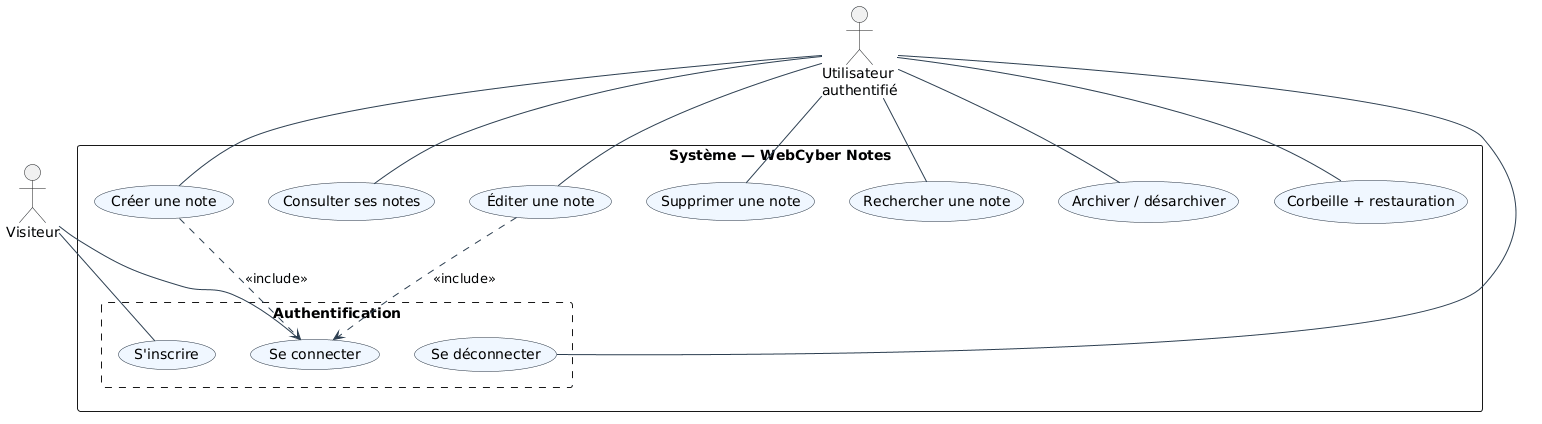
\includegraphics[width=\linewidth]{figures/img/fig04-cas-utilisation.png}
  \caption{Diagramme de cas d'utilisation de WebCyber.}
  \label{fig:cas-utilisation}
\end{figure}

\section{Besoins non fonctionnels}

Les besoins non fonctionnels traduisent les \emph{qualités attendues}
du système, indépendamment des fonctionnalités elles-mêmes.

\subsection{Sécurité}

\begin{itemize}
  \item \textbf{Confidentialité} : tout le trafic entre le client et le
        serveur doit être chiffré (HTTPS, TLS 1.2 ou 1.3).
  \item \textbf{Authentification forte} : les mots de passe ne sont
        jamais stockés en clair; un algorithme de hachage à coût
        configurable (PBKDF2-SHA256) est utilisé.
  \item \textbf{Protection contre les vulnérabilités OWASP Top 10} :
        en particulier les injections SQL, le XSS, le CSRF et les
        contournements de contrôle d'accès.
  \item \textbf{Isolation réseau} : seuls les ports strictement
        nécessaires (22, 80, 443) sont exposés au public.
  \item \textbf{Isolation des données} : un utilisateur ne peut en
        aucun cas accéder aux notes d'un autre.
\end{itemize}

\subsection{Disponibilité et performance}

\begin{itemize}
  \item \textbf{Disponibilité} : le projet ne vise pas la haute
        disponibilité; une instance EC2 unique suffit. Le redémarrage
        automatique des conteneurs (\texttt{restart: unless-stopped})
        couvre les pannes logicielles.
  \item \textbf{Performance} : la solution doit pouvoir servir une
        dizaine d'utilisateurs simultanés sur une instance \texttt{t2.micro}
        (1~vCPU, 1~Gio de RAM). Cela correspond largement aux besoins
        d'une démonstration ou d'un usage personnel.
\end{itemize}

\subsection{Déploiement et maintenabilité}

\begin{itemize}
  \item \textbf{Déploiement reproductible} : la solution doit pouvoir
        être redéployée \emph{from scratch} à partir du dépôt Git, en
        moins de trente minutes.
  \item \textbf{Conteneurisation complète} : aucun composant n'est
        installé directement sur l'hôte; tout passe par Docker
        Compose.
  \item \textbf{Documentation} : l'ensemble des choix d'architecture,
        de configuration et de sécurité est documenté de manière à
        permettre à un autre étudiant ou ingénieur de prendre la suite.
  \item \textbf{Renouvellement automatisé} des certificats TLS via
        Certbot (cron quotidien).
\end{itemize}

\subsection{Ergonomie}

\begin{itemize}
  \item Interface web responsive (mobile et desktop), basée sur
        \textbf{Tailwind CSS} pour un rendu moderne et cohérent.
  \item Navigation simple : barre latérale pour basculer entre la
        liste, l'archive et la corbeille; palette de commandes pour
        un accès rapide.
\end{itemize}

\subsection{Périmètre exclu}

Pour rester fidèle au cadre académique du PFE, certains éléments
classiques d'une production réelle sont \textbf{volontairement exclus} :

\begin{itemize}
  \item Orchestration Kubernetes ou multi-instance (\emph{auto-scaling});
  \item Pipeline CI/CD complet (GitHub Actions \(+\) déploiement
        automatique);
  \item \emph{Web Application Firewall}, services de protection AWS
        avancés (WAF, GuardDuty);
  \item Centralisation des journaux (CloudWatch, ELK);
  \item Monitoring applicatif (Prometheus, Grafana).
\end{itemize}

Ces éléments sont mentionnés dans la \textbf{conclusion générale}
comme perspectives d'évolution.

\section{Conclusion du chapitre}

L'analyse des besoins fait ressortir un système fonctionnellement
simple mais soumis à des exigences non fonctionnelles
\emph{nombreuses} (sécurité, déploiement reproductible, isolation,
HTTPS). Le chapitre suivant traduit ces exigences en une architecture
concrète : choix de l'infrastructure AWS, organisation des conteneurs
Docker, modèle de données, conception de la sécurité en profondeur.

\chapter{Conception}

\section*{Introduction}

Ce chapitre traduit les besoins du chapitre précédent en une
\textbf{architecture technique} précise. Il présente d'abord
l'architecture globale du système, puis l'infrastructure AWS et
l'architecture Docker, le modèle de données, plusieurs scénarios
d'interaction (diagrammes de séquence) et enfin la conception de la
sécurité \textbf{en profondeur}.

\section{Architecture globale}

L'architecture cible peut être résumée par la figure
\ref{fig:archi-globale}. Le navigateur du client résout d'abord le
nom de domaine \texttt{webcyber.app} via Route\,53, qui retourne
l'\textbf{Elastic IP} de l'instance EC2. La requête HTTPS atteint
ensuite l'instance, où elle traverse le \textbf{Security Group} avant
d'être servie par le conteneur Nginx, qui terminera TLS et
\emph{proxifiera} la requête vers l'application Flask.

\begin{figure}[H]
  \centering
  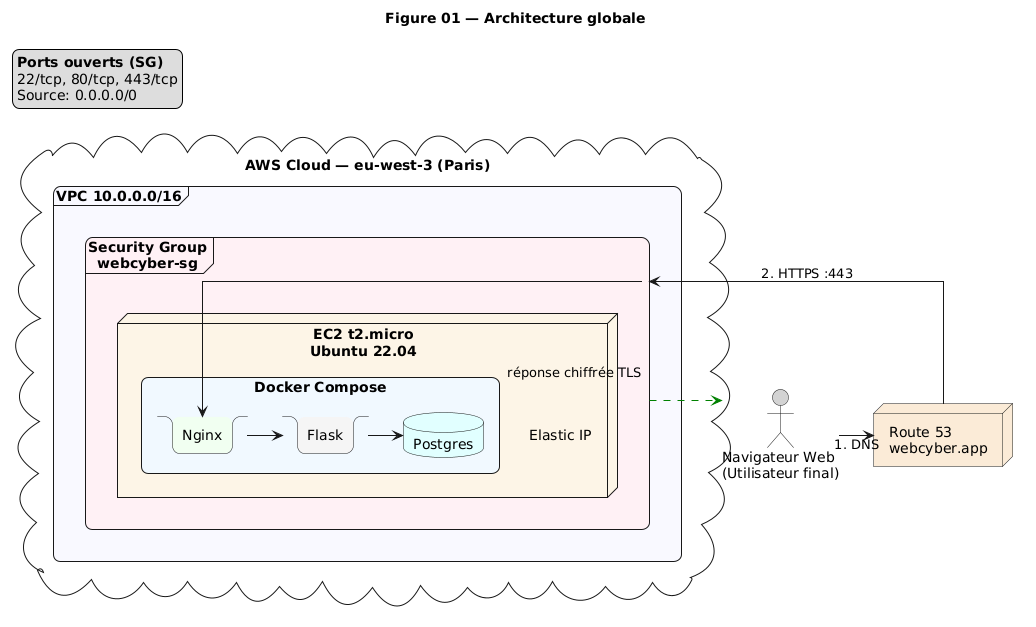
\includegraphics[width=\linewidth]{figures/img/fig01-architecture-globale.png}
  \caption{Architecture globale --- vue d'ensemble.}
  \label{fig:archi-globale}
\end{figure}

\subsection{Composants et responsabilités}

\begin{longtable}{P{3cm} P{11cm}}
\toprule
\textbf{Composant} & \textbf{Responsabilité} \\
\midrule
\endhead
Route\,53        & Résolution DNS : \texttt{webcyber.app} \(\to\) Elastic IP. \\
Elastic IP       & Adresse IPv4 publique fixe associée à l'EC2. \\
EC2 (t2.micro)   & Hôte Ubuntu 22.04 exécutant Docker. \\
Security Group   & Pare-feu \emph{stateful} au niveau de l'EC2. \\
Conteneur Nginx  & Proxy inverse, terminaison TLS, en-têtes de sécurité. \\
Conteneur Flask  & Logique applicative, authentification, CRUD. \\
Conteneur PostgreSQL & Persistance des données utilisateur. \\
\bottomrule
\end{longtable}

\section{Infrastructure AWS}

\subsection{Choix de la région}

La région \texttt{eu-west-3} (Paris) a été choisie pour sa proximité
géographique (latence réduite vers la Mauritanie et l'Europe
francophone) et pour des considérations de \emph{résidence des données}
(stockage en Europe).

\subsection{Composants AWS retenus}

La figure \ref{fig:aws-infra} détaille l'organisation interne au
\emph{cloud}. Les choix retenus privilégient la \textbf{simplicité} et
la \textbf{lisibilité} pédagogique :

\begin{itemize}
  \item utilisation du \textbf{VPC par défaut} (CIDR
        \texttt{172.31.0.0/16}) sans VPC personnalisé;
  \item un \textbf{sous-réseau public} unique;
  \item un \textbf{Security Group dédié} (\texttt{webcyber-sg});
  \item une seule \textbf{instance EC2} \texttt{t2.micro};
  \item une \textbf{Elastic IP} associée;
  \item une \textbf{zone hébergée Route\,53} pour le domaine
        \texttt{webcyber.app}.
\end{itemize}

\begin{figure}[H]
  \centering
  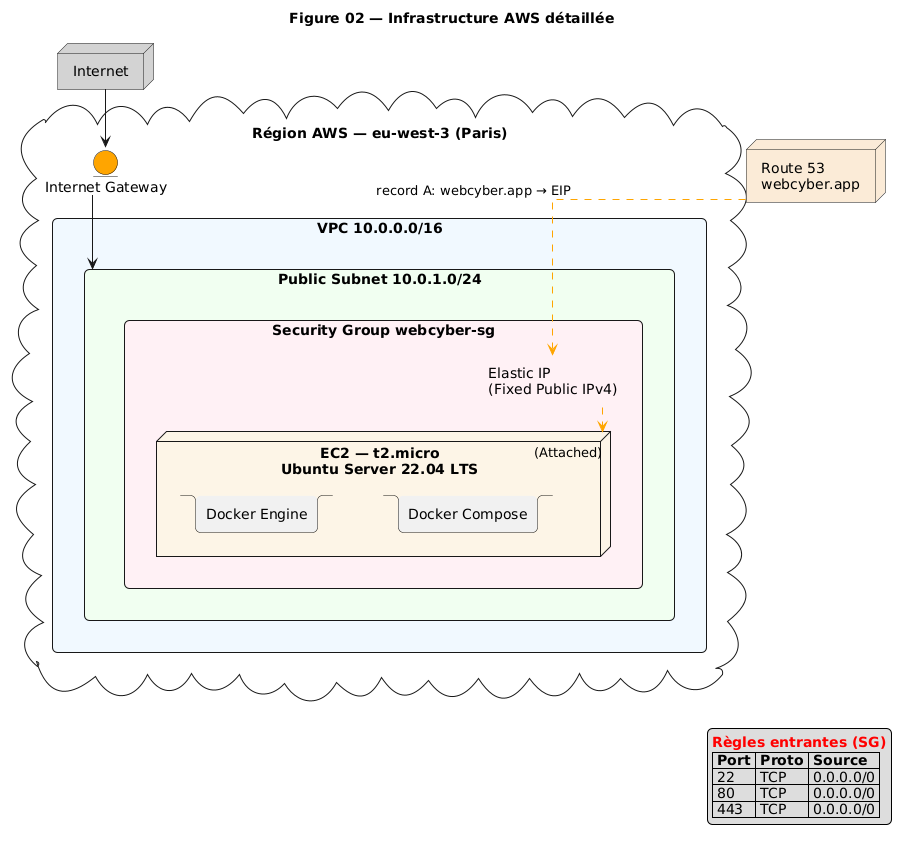
\includegraphics[width=\linewidth]{figures/img/fig02-aws-infrastructure.png}
  \caption{Infrastructure AWS détaillée.}
  \label{fig:aws-infra}
\end{figure}

\subsection{Règles du Security Group}

Le pare-feu réseau du périmètre est un \textbf{Security Group}
\emph{stateful} : seul le trafic entrant explicitement autorisé est
accepté, et les réponses correspondantes sont automatiquement
autorisées en sortie.

\begin{table}[H]
\centering
\caption{Règles entrantes du Security Group \texttt{webcyber-sg}.}
\begin{tabular}{C{2cm} C{2cm} C{1.5cm} P{4cm} P{4cm}}
\toprule
\textbf{Type} & \textbf{Protocole} & \textbf{Port} & \textbf{Source} & \textbf{Justification} \\
\midrule
SSH   & TCP & 22  & \texttt{0.0.0.0/0} & Administration distante \\
HTTP  & TCP & 80  & \texttt{0.0.0.0/0} & Redirection vers HTTPS \\
HTTPS & TCP & 443 & \texttt{0.0.0.0/0} & Trafic web chiffré \\
\bottomrule
\end{tabular}
\end{table}

Aucun autre port n'est ouvert. Les ports applicatifs (\texttt{5000}
pour Flask, \texttt{5432} pour PostgreSQL) restent confinés au réseau
Docker interne et ne sont donc pas accessibles depuis Internet.

\subsection{Estimation des coûts}

\begin{table}[H]
\centering
\caption{Estimation mensuelle (sous \emph{free tier} AWS).}
\begin{tabular}{P{6cm} R{3cm}}
\toprule
\textbf{Ressource} & \textbf{Coût} \\
\midrule
EC2 \texttt{t2.micro}            & \$0,00 \\
EBS 20~Gio gp3                   & \$0,00 \\
Elastic IP (associée)            & \$0,00 \\
Route\,53 zone hébergée          & \$0,50 \\
Trafic sortant (faible)          & $\approx$ \$0,00 \\
\midrule
\textbf{Total estimé}            & $\approx$ \textbf{\$0,50/mois} \\
\bottomrule
\end{tabular}
\end{table}

\section{Architecture Docker}

\subsection{Vue d'ensemble}

Trois conteneurs cohabitent sur l'instance, orchestrés par Docker
Compose et reliés par un réseau \emph{bridge} privé
(\texttt{webcyber-net}). La figure \ref{fig:docker-archi} montre cette
organisation, ainsi que les volumes persistants utilisés.

\begin{figure}[H]
  \centering
  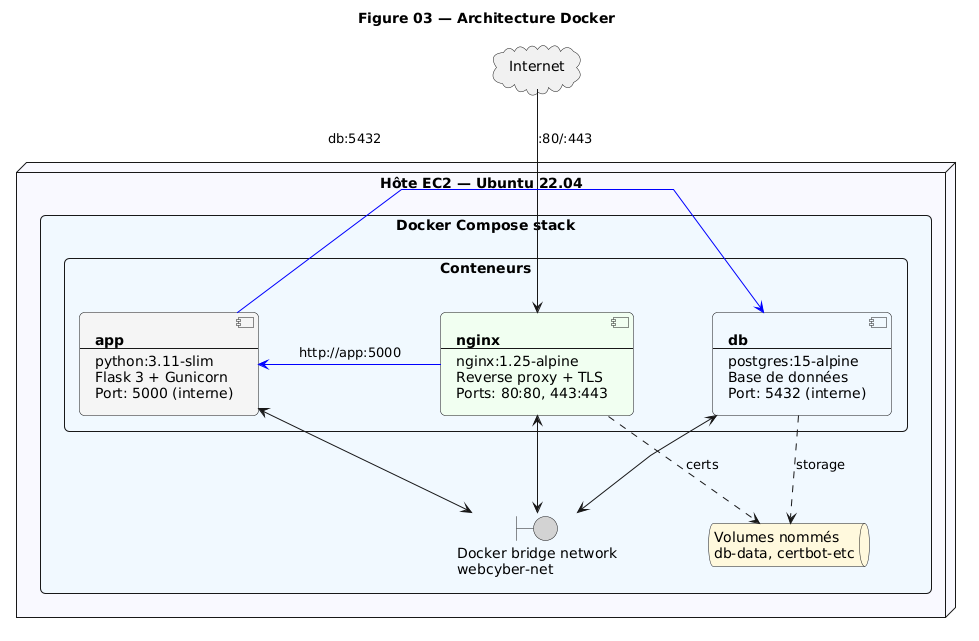
\includegraphics[width=\linewidth]{figures/img/fig03-docker-architecture.png}
  \caption{Architecture Docker --- trois conteneurs sur réseau \emph{bridge}.}
  \label{fig:docker-archi}
\end{figure}

\subsection{Spécifications des conteneurs}

\begin{longtable}{P{2cm} P{5cm} P{2.5cm} P{4cm}}
\toprule
\textbf{Service} & \textbf{Image} & \textbf{Ports} & \textbf{Rôle} \\
\midrule
\endhead
\texttt{nginx} & \texttt{nginx:1.25-alpine} & 80, 443 (publiés) & Proxy inverse, TLS, en-têtes de sécurité \\
\texttt{app}   & \texttt{python:3.11-slim} (build) & 5000 (interne) & Application Flask + Gunicorn \\
\texttt{db}    & \texttt{postgres:15-alpine} & 5432 (interne) & Base de données PostgreSQL \\
\bottomrule
\end{longtable}

Le \emph{principe d'exposition minimale} est appliqué : seul le proxy
publie ses ports vers l'hôte. Les services \texttt{app} et \texttt{db}
ne sont accessibles qu'\emph{intra-Docker}, par leur nom de service
(résolution DNS embarquée par Docker).

\subsection{Volumes persistants}

\begin{itemize}
  \item \texttt{db-data} : données PostgreSQL (table \texttt{users},
        table \texttt{notes}, indexes, WAL).
  \item \texttt{certbot-etc} : certificats Let's Encrypt et clés
        privées.
  \item \texttt{certbot-var} : état interne de Certbot (compte ACME,
        \emph{lock files}).
\end{itemize}

\subsection{Estimation des ressources}

Sur \texttt{t2.micro} (1~Gio RAM), l'occupation mémoire prévisionnelle
est confortable :

\begin{table}[H]
\centering
\caption{Empreinte mémoire estimée des conteneurs.}
\begin{tabular}{P{4cm} R{4cm}}
\toprule
\textbf{Conteneur}   & \textbf{Mémoire estimée} \\
\midrule
Nginx                & 10--30 Mio \\
Flask + 2 \emph{workers} Gunicorn & 100--200 Mio \\
PostgreSQL           & 50--100 Mio \\
Surcharge Docker     & $\approx$ 100 Mio \\
\midrule
\textbf{Total}       & $\approx$ \textbf{300--430 Mio} \\
\bottomrule
\end{tabular}
\end{table}

\section{Modèle de données}

Le modèle de données est volontairement réduit à deux entités, comme
le montre la figure \ref{fig:classes}.

\begin{figure}[H]
  \centering
  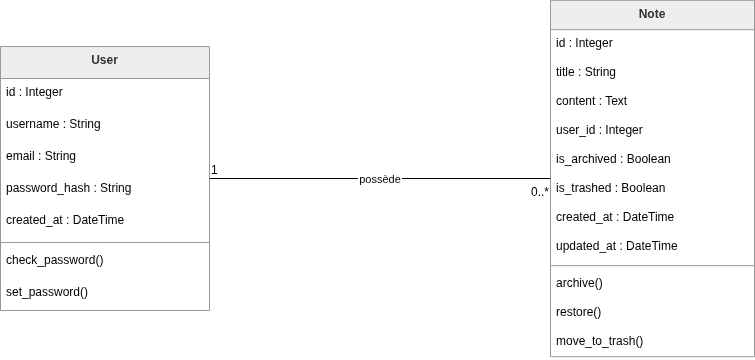
\includegraphics[width=0.95\linewidth]{figures/img/fig05-diagramme-classes.png}
  \caption{Diagramme de classes (modèle de données).}
  \label{fig:classes}
\end{figure}

\subsection{Description}

\begin{itemize}
  \item Un \textbf{User} possède de zéro à $n$ \textbf{Notes}.
  \item Une \textbf{Note} appartient à exactement un \textbf{User}, via
        la clé étrangère \texttt{user\_id}.
  \item Les drapeaux \texttt{is\_archived} et \texttt{is\_trashed}
        permettent une suppression \emph{douce} (corbeille) et une
        archive sans déplacer ni dupliquer la donnée.
\end{itemize}

\subsection{Considérations de sécurité dans le modèle}

\begin{itemize}
  \item Le champ \texttt{password\_hash} contient uniquement le
        \emph{hachage} du mot de passe, jamais sa valeur en clair.
  \item Les contraintes \texttt{UNIQUE} sur \texttt{username} et
        \texttt{email} préviennent les doublons et certaines attaques
        d'énumération.
  \item Toutes les requêtes \texttt{SELECT}, \texttt{UPDATE} ou
        \texttt{DELETE} sur la table \texttt{notes} \textbf{doivent}
        comporter le filtre \texttt{WHERE user\_id = current\_user.id}.
\end{itemize}

\section{Diagrammes de séquence}

\subsection{Authentification}

Le scénario d'authentification met en jeu cinq acteurs : l'utilisateur,
son navigateur, Nginx, Flask et PostgreSQL. La figure
\ref{fig:seq-auth} en détaille le déroulement, depuis la saisie des
identifiants jusqu'à la création de la session côté serveur et au
positionnement du \emph{cookie} dans le navigateur.

\begin{figure}[H]
  \centering
  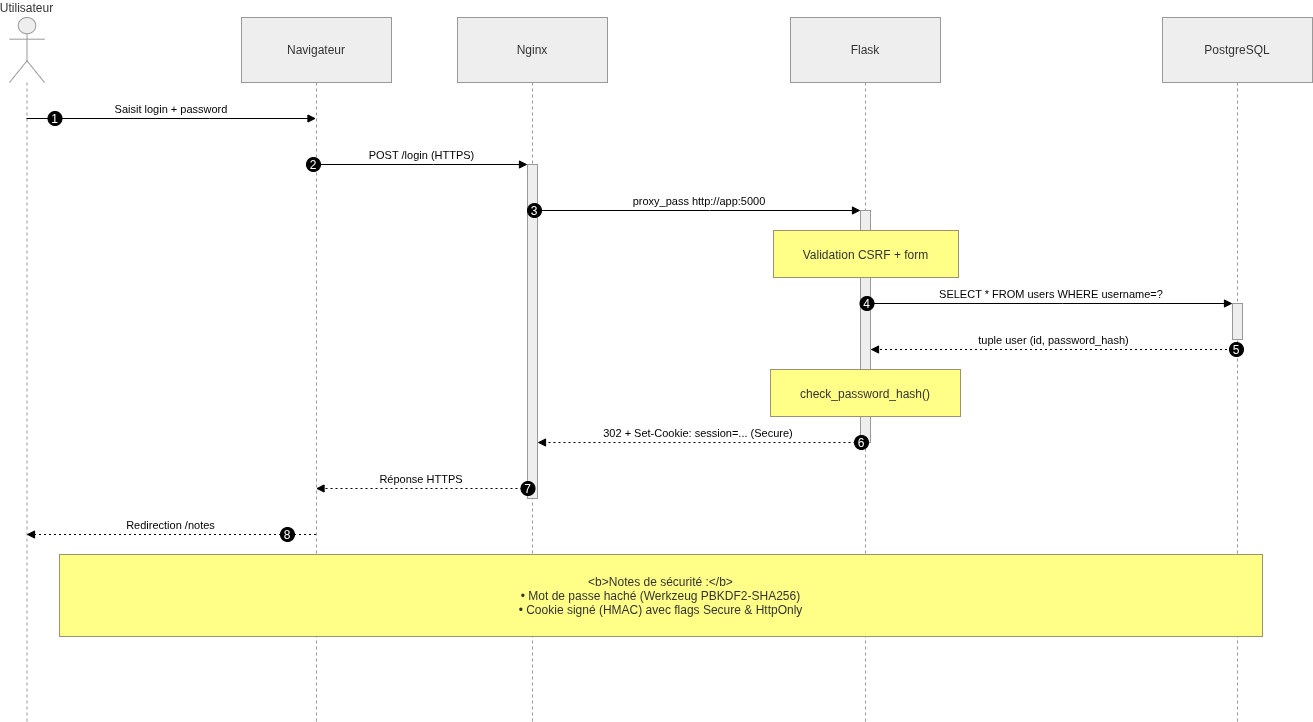
\includegraphics[width=\linewidth]{figures/img/fig06-sequence-authentification.png}
  \caption{Diagramme de séquence --- authentification.}
  \label{fig:seq-auth}
\end{figure}

Trois éléments de sécurité sont à noter :

\begin{enumerate}
  \item le mot de passe ne quitte jamais le tunnel TLS;
  \item la comparaison côté serveur passe par
        \texttt{check\_password\_hash}, qui exécute une comparaison
        \emph{constant-time};
  \item le \emph{cookie} de session est signé (HMAC), et porte les
        attributs \texttt{Secure}, \texttt{HttpOnly} et
        \texttt{SameSite=Lax}.
\end{enumerate}

\subsection{Création d'une note}

Le scénario de création d'une note (figure \ref{fig:seq-note}) montre
en particulier le contrôle de session
(\texttt{@login\_required}), la vérification du jeton CSRF, puis
l'insertion en base avec association à l'utilisateur courant.

\begin{figure}[H]
  \centering
  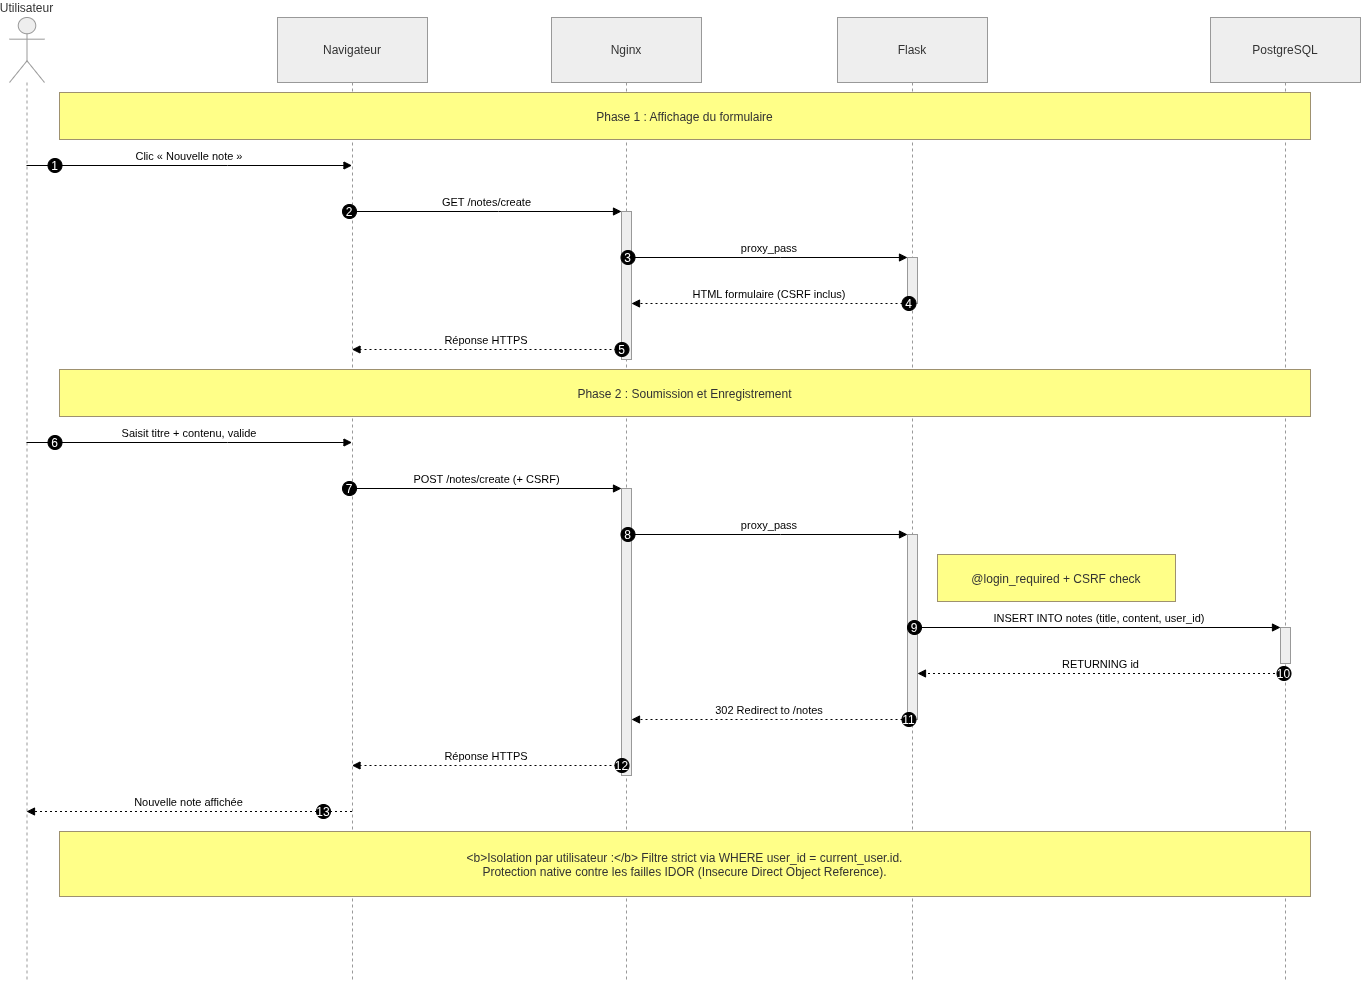
\includegraphics[width=\linewidth]{figures/img/fig07-sequence-note.png}
  \caption{Diagramme de séquence --- création d'une note.}
  \label{fig:seq-note}
\end{figure}

\section{Conception de la sécurité --- défense en profondeur}

La sécurité du système ne repose pas sur une unique mesure, mais sur
\textbf{six couches empilées}, chacune apportant une garantie
spécifique. La figure \ref{fig:couches-securite} en donne une
représentation synthétique.

\begin{figure}[H]
  \centering
  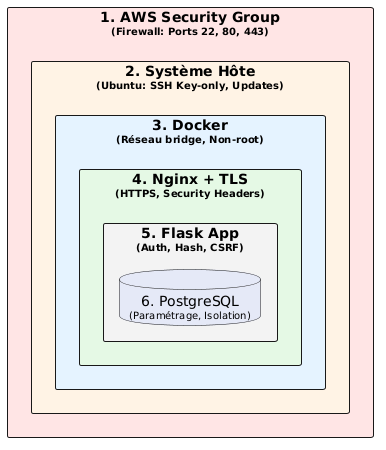
\includegraphics[width=\linewidth]{figures/img/fig09-couches-securite.png}
  \caption{Les six couches de sécurité (\emph{defense-in-depth}).}
  \label{fig:couches-securite}
\end{figure}

\subsection{Couche 1 --- Security Group}

Le Security Group AWS est un pare-feu \emph{stateful} qui constitue la
\textbf{première ligne de défense} : il bloque tout port non
explicitement autorisé. Sa configuration a été détaillée plus haut.

\subsection{Couche 2 --- Système hôte}

Sur l'instance EC2 :

\begin{itemize}
  \item \texttt{PermitRootLogin no} : interdiction du login SSH
        \texttt{root};
  \item authentification SSH par clé en mode primaire;
  \item \texttt{unattended-upgrades} pour appliquer les mises à jour
        de sécurité automatiquement;
  \item utilisateur applicatif \texttt{ubuntu} non-root.
\end{itemize}

\subsection{Couche 3 --- Isolation Docker}

\begin{itemize}
  \item Réseau \emph{bridge} privé \texttt{webcyber-net}; les
        conteneurs \texttt{app} et \texttt{db} ne publient pas de
        port;
  \item Le \emph{Dockerfile} de l'application crée un utilisateur
        non-privilégié \texttt{appuser} (UID 1000) et l'utilise pour
        l'exécution finale;
  \item Les volumes nommés isolent les données persistantes du système
        de fichiers de l'hôte.
\end{itemize}

\subsection{Couche 4 --- Nginx + TLS}

\begin{itemize}
  \item TLS 1.2 et 1.3 uniquement, profil \emph{Mozilla Intermediate};
  \item certificat \textbf{Let's Encrypt} renouvelé automatiquement;
  \item redirection \(80 \to 443\);
  \item en-têtes \textbf{HSTS}, \textbf{CSP}, \textbf{X-Frame-Options},
        \textbf{X-Content-Type-Options}, \textbf{Referrer-Policy}
        injectés sur toutes les réponses;
  \item \texttt{server\_tokens off} pour masquer la version de Nginx.
\end{itemize}

\subsection{Couche 5 --- Application Flask}

\begin{itemize}
  \item Hachage des mots de passe via
        \texttt{generate\_password\_hash} (PBKDF2-SHA256, sel
        automatique);
  \item Session signée par \texttt{SECRET\_KEY} aléatoire (32 octets);
  \item Protection \textbf{CSRF} sur tous les formulaires (Flask-WTF);
  \item Validation systématique des entrées par WTForms (longueur,
        type, présence);
  \item Décorateur \texttt{@login\_required} sur toutes les routes
        privées;
  \item Filtre \texttt{user\_id} sur 100\,\% des requêtes \emph{notes}.
\end{itemize}

\subsection{Couche 6 --- Base de données}

\begin{itemize}
  \item Utilisateur \texttt{webcyber\_user} non-superutilisateur;
  \item Mot de passe long et aléatoire (>=20 caractères) injecté via
        \texttt{.env};
  \item Pas de port publié vers l'hôte;
  \item Requêtes paramétrées par SQLAlchemy (pas de concaténation de
        chaînes SQL).
\end{itemize}

\section{Conclusion du chapitre}

La conception ainsi décrite est volontairement \emph{minimale mais
complète} : un seul serveur, trois conteneurs, deux entités, mais une
sécurité empilée sur six niveaux. Le chapitre suivant présente la
réalisation concrète de cette conception et les étapes de son
déploiement.

\chapter{Réalisation et déploiement}

\section*{Introduction}

Ce chapitre décrit la réalisation concrète de l'application
WebCyber : choix technologiques détaillés, construction des images
Docker, configuration de l'instance EC2, mise en place du DNS via
Route\,53, configuration de Nginx avec HTTPS Let's Encrypt, et
procédure de déploiement \textit{from scratch}. Il se termine par le
diagramme de déploiement UML qui synthétise l'ensemble.

\section{Environnement et outils}

\subsection{Poste de développement}

\begin{itemize}
  \item OS : Linux (Ubuntu 24.04);
  \item IDE : Visual Studio Code;
  \item Outils en ligne de commande : \texttt{git}, \texttt{docker},
        \texttt{docker compose}, \texttt{terraform}, \texttt{tfsec},
        \texttt{ssh}, \texttt{curl}, \texttt{dig};
  \item Gestionnaire de versions : Git, dépôt distant sur GitHub.
\end{itemize}

\subsection{Stack technologique retenue}

\begin{table}[H]
\centering
\caption{Synthèse de la pile technologique.}
\begin{tabular}{P{3.5cm} P{4cm} P{6.5cm}}
\toprule
\textbf{Couche} & \textbf{Choix} & \textbf{Justification} \\
\midrule
Cloud / IaaS    & AWS EC2          & Standard du marché, \emph{free tier}, riche écosystème. \\
Système         & Ubuntu 24.04 LTS & LTS, large support Docker. \\
IaC             & Terraform 1.12 + provider AWS 5.98 & Provisionnement déclaratif et reproductible de l'infra. \\
Conteneurs      & Docker + Compose & Reproductibilité, isolation. \\
Registre images & GitHub Container Registry (GHCR) & Distribution de l'image applicative. \\
CI/CD           & GitHub Actions   & Pipeline build / scan / déploiement automatisé. \\
Sécurité IaC    & tfsec (Aqua)     & Analyse statique du code Terraform (\textit{SAST} infra). \\
Proxy / TLS     & Nginx 1.25       & Léger, robuste, terminaison TLS éprouvée. \\
Langage         & Python 3.11      & Productivité, écosystème mature. \\
Framework web   & Flask 3          & Léger, transparent, pédagogique. \\
WSGI            & Gunicorn         & WSGI de production, multi-\emph{worker}. \\
ORM             & SQLAlchemy 2     & Empêche par construction l'injection SQL. \\
Auth            & Flask-Login      & Gestion de session simple et bien testée. \\
Formulaires     & Flask-WTF        & Validation \(+\) CSRF intégrée. \\
Hash mot de passe & Werkzeug PBKDF2-SHA256 & Sel automatique, coût configurable. \\
Base de données & PostgreSQL 16    & Robuste, indexation et JSON natifs. \\
TLS / CA        & Let's Encrypt + Certbot & Certificats gratuits et automatiques. \\
Front-end       & Tailwind CSS     & Mise en page rapide et responsive. \\
\bottomrule
\end{tabular}
\end{table}

\section{Implémentation de l'application Flask}

\subsection{Organisation du code}

Le code source de l'application est structuré selon le \emph{pattern}
\textbf{application factory} de Flask, qui sépare la création de
l'application, les \emph{blueprints} (groupes de routes) et les modèles
de données.

\begin{lstlisting}[language=bash, caption={Arborescence de l'application Flask.}]
app/
├── Dockerfile
├── requirements.txt
├── wsgi.py             # point d'entree Gunicorn
├── config.py           # lecture de l'environnement
├── app.py              # create_app(), init des extensions
├── models.py           # User, Note (SQLAlchemy)
├── forms.py            # LoginForm, RegisterForm, NoteForm
├── routes/
│   ├── auth.py         # /login, /register, /logout
│   └── notes.py        # CRUD, archive, corbeille, recherche
├── templates/          # Jinja2 (auto-escape par defaut)
└── static/             # CSS, JS, images
\end{lstlisting}

\subsection{Modèles SQLAlchemy}

\begin{lstlisting}[language=Python, caption={Extrait de \texttt{models.py}.}]
from flask_sqlalchemy import SQLAlchemy
from werkzeug.security import generate_password_hash, check_password_hash
from flask_login import UserMixin

db = SQLAlchemy()

class User(UserMixin, db.Model):
    __tablename__ = "users"
    id            = db.Column(db.Integer, primary_key=True)
    username      = db.Column(db.String(80),  unique=True, nullable=False)
    email         = db.Column(db.String(120), unique=True, nullable=False)
    password_hash = db.Column(db.String(256), nullable=False)
    created_at    = db.Column(db.DateTime, default=db.func.now())
    notes         = db.relationship("Note", backref="owner", lazy=True)

    def set_password(self, password):
        self.password_hash = generate_password_hash(
            password, method="pbkdf2:sha256"
        )

    def check_password(self, password):
        return check_password_hash(self.password_hash, password)


class Note(db.Model):
    __tablename__ = "notes"
    id           = db.Column(db.Integer, primary_key=True)
    title        = db.Column(db.String(200), nullable=False)
    content      = db.Column(db.Text,       nullable=False)
    user_id      = db.Column(db.Integer, db.ForeignKey("users.id"),
                              nullable=False)
    is_archived  = db.Column(db.Boolean, default=False)
    is_trashed   = db.Column(db.Boolean, default=False)
    created_at   = db.Column(db.DateTime, default=db.func.now())
    updated_at   = db.Column(db.DateTime, default=db.func.now(),
                              onupdate=db.func.now())
\end{lstlisting}

\subsection{Authentification et isolation}

\begin{lstlisting}[language=Python, caption={Extrait du \emph{blueprint} \texttt{notes.py} --- isolation par utilisateur.}]
from flask import Blueprint, request, render_template, redirect, url_for
from flask_login import login_required, current_user
from .models import db, Note

notes_bp = Blueprint("notes", __name__, url_prefix="/notes")

@notes_bp.route("/")
@login_required
def list_notes():
    # Filtre systematique par user_id : isolation des donnees
    notes = (Note.query
                 .filter_by(user_id=current_user.id, is_trashed=False)
                 .order_by(Note.updated_at.desc())
                 .all())
    return render_template("notes/list.html", notes=notes)

@notes_bp.route("/<int:note_id>")
@login_required
def view_note(note_id):
    # 404 si la note n'appartient pas a l'utilisateur courant
    note = (Note.query
                .filter_by(id=note_id, user_id=current_user.id)
                .first_or_404())
    return render_template("notes/view.html", note=note)
\end{lstlisting}

Le \texttt{filter\_by(user\_id=current\_user.id)} sur \emph{toutes} les
requêtes garantit qu'un utilisateur ne peut pas accéder aux notes d'un
autre, même en forgeant un identifiant dans l'URL (parade contre
l'\textbf{IDOR}).

\section{Conteneurisation}

\subsection{Dockerfile applicatif}

\begin{lstlisting}[language=bash, caption={\texttt{app/Dockerfile}.}]
FROM python:3.11-slim

# Securite : utilisateur non-root
RUN useradd -m -u 1000 appuser

WORKDIR /app

# Dependances
COPY requirements.txt .
RUN pip install --no-cache-dir -r requirements.txt

# Code applicatif
COPY . .
RUN chown -R appuser:appuser /app

USER appuser

EXPOSE 5000

# WSGI de production
CMD ["gunicorn", "--bind", "0.0.0.0:5000", "--workers", "2", "wsgi:app"]
\end{lstlisting}

Trois bonnes pratiques sont appliquées : (i)~image \emph{slim} pour
réduire la surface d'attaque, (ii)~création d'un utilisateur
\texttt{appuser} non-root, (iii)~Gunicorn comme serveur WSGI au lieu
du serveur de développement de Flask.

\subsection{Fichier docker-compose.yml}

\begin{lstlisting}[language=bash, caption={\texttt{docker-compose.yml} --- vue conceptuelle.}]
version: "3.8"

services:
  nginx:
    image: nginx:1.25-alpine
    depends_on: [app]
    ports:
      - "80:80"
      - "443:443"
    volumes:
      - ./nginx/nginx.conf:/etc/nginx/nginx.conf:ro
      - ./nginx/conf.d/:/etc/nginx/conf.d/:ro
      - certbot-etc:/etc/letsencrypt
      - certbot-var:/var/lib/letsencrypt
      - ./app/static/:/usr/share/nginx/static/:ro
    restart: unless-stopped
    networks: [webcyber-net]

  app:
    build: ./app
    depends_on: [db]
    env_file: .env
    restart: unless-stopped
    networks: [webcyber-net]

  db:
    image: postgres:15-alpine
    env_file: .env
    volumes:
      - db-data:/var/lib/postgresql/data
    restart: unless-stopped
    networks: [webcyber-net]

networks:
  webcyber-net:
    driver: bridge

volumes:
  db-data:
  certbot-etc:
  certbot-var:
\end{lstlisting}

\section{Infrastructure as Code avec Terraform}

\subsection{Motivation}

Plutôt que de provisionner l'infrastructure manuellement via la console
AWS \---\ démarche peu reproductible et sujette à l'erreur humaine \---,
l'infrastructure est décrite \textbf{en code} avec
\textbf{Terraform}~5.98. Cette approche, dite \emph{Infrastructure as
Code (IaC)}, présente plusieurs avantages :

\begin{itemize}
  \item \textbf{Reproductibilité} : la même configuration peut être
        rejouée à l'identique, en local comme en CI/CD;
  \item \textbf{Versionnement} : le code Terraform est versionné dans
        Git aux côtés du code applicatif;
  \item \textbf{Auditabilité} : chaque modification d'infrastructure
        passe par une \emph{pull request} et un plan d'exécution
        (\texttt{terraform plan}) lisible en revue de code;
  \item \textbf{Analyse statique} : des outils comme \texttt{tfsec}
        peuvent inspecter le code et détecter les mauvaises
        configurations \emph{avant} le déploiement (cf.
        chapitre~\ref{chap:tests}).
\end{itemize}

\subsection{Organisation des fichiers}

\begin{lstlisting}[language=bash, caption={Arborescence du module Terraform.}]
terraform/
|-- provider.tf      # bloc terraform + provider AWS
|-- main.tf          # ressources : data AMI, SG, EC2, EIP association
|-- variables.tf     # declarations de variables
|-- dev.tfvars       # valeurs (gitignore)
|-- vockey.pem       # cle SSH d'AWS Academy (gitignore, chmod 400)
\end{lstlisting}

\subsection{Bloc Terraform et provider}

\begin{lstlisting}[language=bash, caption={\texttt{provider.tf}.}]
terraform {
  required_version = ">= 1.12.0"
  required_providers {
    aws = { source = "hashicorp/aws", version = "5.98.0" }
  }
}

provider "aws" {
  region = "us-east-1"
}
\end{lstlisting}

\subsection{Ressources principales}

Le fichier \texttt{main.tf} décrit trois ressources et une
\textit{data source} :

\begin{enumerate}
  \item \texttt{data "aws\_ami" "ubuntu"} : recherche dynamique de la
        dernière AMI Ubuntu 24.04 LTS publiée par Canonical;
  \item \texttt{aws\_security\_group "ssh"} : règles entrantes 22, 80,
        443 ouvertes au monde, sortantes libres;
  \item \texttt{aws\_instance "instance"} : EC2 t3.micro, IMDSv2
        forcé, \textit{provisioner} \texttt{remote-exec} qui installe
        Docker \(+\) Compose au premier \texttt{apply};
  \item \texttt{aws\_eip\_association "instance"} : association de
        l'Elastic IP existante (\texttt{eipalloc-...}) à la nouvelle
        instance, afin que le DNS reste valide.
\end{enumerate}

\begin{lstlisting}[language=bash, caption={Extrait de \texttt{main.tf} (ressource EC2).}]
# tfsec:ignore:aws-ec2-enable-at-rest-encryption (lab academique)
resource "aws_instance" "instance" {
  ami             = data.aws_ami.ubuntu.id
  instance_type   = var.instance_type
  security_groups = [aws_security_group.ssh.name]
  key_name        = var.key_name

  metadata_options {
    http_endpoint = "enabled"
    http_tokens   = "required"   # IMDSv2 obligatoire
  }

  provisioner "remote-exec" {
    inline = [
      "sudo apt-get update",
      "curl -fsSL https://get.docker.com | sudo sh",
      "sudo usermod -aG docker ubuntu",
      "sudo systemctl enable --now docker"
    ]
    connection {
      type        = "ssh"
      user        = "ubuntu"
      private_key = file(var.private_key_path)
      host        = self.public_ip
    }
  }
  tags = { Name = var.instance_name }
}
\end{lstlisting}

\subsection{Cycle de provisionnement}

\begin{lstlisting}[language=bash, caption={Commandes Terraform.}]
cd terraform/
terraform init                              # telechargement du provider
terraform plan  -var-file="dev.tfvars"      # plan d'execution
terraform apply -var-file="dev.tfvars"      # creation des ressources
terraform destroy -var-file="dev.tfvars"    # destruction propre
\end{lstlisting}

À la fin de l'\texttt{apply}, Terraform affiche les sorties (\textit{outputs}) :

\begin{lstlisting}[language=bash, caption={Sorties typiques après \texttt{apply}.}]
Apply complete! Resources: 3 added, 0 changed, 0 destroyed.

Outputs:
  public_dns = "ec2-54-165-116-113.compute-1.amazonaws.com"
  public_ip  = "54.165.116.113"
\end{lstlisting}

L'EIP étant associée à l'instance, l'adresse publique reste stable
malgré les redémarrages, ce qui maintient la cohérence des
enregistrements DNS de Route\,53.

\section{Configuration DNS via Route\,53}

Sur Route\,53, une zone hébergée publique est créée pour
\texttt{webcyber.app} et deux enregistrements de type A sont ajoutés :

\begin{table}[H]
\centering
\caption{Enregistrements DNS de la zone hébergée \texttt{webcyber.app}.}
\begin{tabular}{P{4cm} C{1.5cm} C{3cm} C{1.5cm}}
\toprule
\textbf{Nom} & \textbf{Type} & \textbf{Valeur} & \textbf{TTL} \\
\midrule
\texttt{webcyber.app}      & A & \(<\)Elastic IP\(>\) & 300 \\
\texttt{www.webcyber.app}  & A & \(<\)Elastic IP\(>\) & 300 \\
\bottomrule
\end{tabular}
\end{table}

Le TLD \texttt{.app} étant inscrit sur la liste \emph{HSTS preload},
le navigateur \textbf{refuse toute connexion non-HTTPS} : la mise en
place de Let's Encrypt est donc obligatoire.

\section{Préparation automatique de l'instance}

À la différence d'une approche manuelle (\texttt{ssh}, \texttt{apt
install}, configuration ligne par ligne), la préparation de l'EC2
est entièrement automatisée par deux mécanismes complémentaires :

\begin{enumerate}
  \item Le \emph{provisioner} \texttt{remote-exec} de Terraform installe
        Docker et active son service au moment du \texttt{terraform
        apply} (cf. extrait de \texttt{main.tf} ci-dessus);
  \item Le pipeline CI/CD (section suivante) clone le dépôt, écrit le
        fichier \texttt{.env} à partir d'un \emph{secret} GitHub, et
        démarre la pile Docker Compose.
\end{enumerate}

Le fichier \texttt{.env} est ainsi \textbf{généré sur le serveur} à
partir d'un secret stocké dans GitHub Actions et \textbf{n'est jamais
versionné}; il est exclu par \texttt{.gitignore}.

\section{Configuration Nginx et HTTPS}

\subsection{Configuration Nginx}

Le proxy Nginx est configuré en deux blocs :

\begin{lstlisting}[language=bash, caption={Extrait \texttt{nginx/conf.d/webcyber.conf}.}]
# Bloc 1 : redirection HTTP -> HTTPS
server {
    listen 80;
    server_name webcyber.app www.webcyber.app;

    location /.well-known/acme-challenge/ {
        root /var/www/certbot;
    }

    location / {
        return 301 https://webcyber.app$request_uri;
    }
}

# Bloc 2 : serveur HTTPS
server {
    listen 443 ssl http2;
    server_name webcyber.app www.webcyber.app;

    ssl_certificate     /etc/letsencrypt/live/webcyber.app/fullchain.pem;
    ssl_certificate_key /etc/letsencrypt/live/webcyber.app/privkey.pem;
    ssl_protocols       TLSv1.2 TLSv1.3;
    ssl_ciphers         HIGH:!aNULL:!MD5;

    # Masquage de la version de Nginx
    server_tokens off;

    # En-tetes de securite
    add_header Strict-Transport-Security "max-age=31536000; includeSubDomains" always;
    add_header X-Content-Type-Options    "nosniff" always;
    add_header X-Frame-Options           "SAMEORIGIN" always;
    add_header Referrer-Policy           "strict-origin-when-cross-origin" always;
    add_header Content-Security-Policy   "default-src 'self'; script-src 'self' 'unsafe-inline'; style-src 'self' 'unsafe-inline'; img-src 'self' data:; font-src 'self' data:; object-src 'none'; base-uri 'self'; frame-ancestors 'self'" always;

    # Tout le trafic : proxy vers Flask
    location / {
        proxy_pass         http://app:5000;
        proxy_set_header   Host              $host;
        proxy_set_header   X-Real-IP         $remote_addr;
        proxy_set_header   X-Forwarded-For   $proxy_add_x_forwarded_for;
        proxy_set_header   X-Forwarded-Proto $scheme;
    }
}
\end{lstlisting}

\paragraph{Détail des en-têtes.}

\begin{table}[H]
\centering
\caption{En-têtes de sécurité HTTP appliqués par Nginx.}
\begin{tabular}{P{4.5cm} P{9cm}}
\toprule
\textbf{En-tête} & \textbf{Rôle} \\
\midrule
\texttt{Strict-Transport-Security} & Force le navigateur à utiliser HTTPS pendant un an (HSTS). \\
\texttt{X-Content-Type-Options}    & Empêche le \textit{MIME-sniffing} (\texttt{nosniff}). \\
\texttt{X-Frame-Options}           & Bloque l'inclusion en \texttt{<iframe>} sauf en \emph{same-origin} (anti-\textit{clickjacking}). \\
\texttt{Referrer-Policy}           & Limite la fuite d'URL via le \emph{referer}. \\
\texttt{Content-Security-Policy}   & Restreint les sources de scripts, styles, images, polices, \ldots\ (défense contre XSS). \\
\texttt{server\_tokens off}        & N'affiche pas la version de Nginx dans les en-têtes (réduction de la divulgation d'information). \\
\bottomrule
\end{tabular}
\end{table}

\subsection{Durcissement des cookies de session Flask}

En complément des en-têtes HTTP, la configuration Flask
(\texttt{app/config.py}) durcit les attributs des cookies de session :

\begin{lstlisting}[language=Python, caption={Extrait de \texttt{config.py} --- cookies de session.}]
class Config:
    FLASK_ENV = os.getenv("FLASK_ENV", "development")

    SESSION_COOKIE_SECURE   = FLASK_ENV == "production"  # cookie envoye uniquement en HTTPS
    SESSION_COOKIE_HTTPONLY = True                       # inaccessible au JavaScript
    SESSION_COOKIE_SAMESITE = "Lax"                      # protection CSRF de base
\end{lstlisting}

Ces trois attributs (\texttt{Secure}, \texttt{HttpOnly},
\texttt{SameSite=Lax}) sont effectivement présents dans la réponse
HTTP, ce qui sera vérifié au chapitre \ref{chap:tests}.

\subsection{Obtention du certificat Let's Encrypt}

L'obtention du certificat suit la méthode \emph{webroot} :

\begin{lstlisting}[language=bash, caption={Première émission du certificat via Certbot.}]
docker run --rm \
  -v certbot-etc:/etc/letsencrypt \
  -v certbot-var:/var/lib/letsencrypt \
  -v ./certbot-webroot:/var/www/certbot \
  certbot/certbot certonly \
  --webroot -w /var/www/certbot \
  -d webcyber.app -d www.webcyber.app \
  --email contact@webcyber.app \
  --agree-tos --no-eff-email
\end{lstlisting}

Une tâche \texttt{cron} quotidienne est ensuite ajoutée pour le
renouvellement automatique :

\begin{lstlisting}[language=bash, caption={Renouvellement automatique des certificats.}]
0 3 * * * cd /home/ubuntu/webcyber && \
  docker run --rm \
    -v certbot-etc:/etc/letsencrypt \
    -v certbot-var:/var/lib/letsencrypt \
    -v ./certbot-webroot:/var/www/certbot \
    certbot/certbot renew --quiet && \
  docker compose exec nginx nginx -s reload
\end{lstlisting}

\subsection{Démarrage de la pile}

En production, la pile est démarrée par le pipeline CI/CD (section
suivante). En local, les commandes suivantes suffisent :

\begin{lstlisting}[language=bash, caption={Démarrage et vérification.}]
docker compose up --build -d
docker compose ps
docker compose logs -f
\end{lstlisting}

\section{Pipeline CI/CD avec GitHub Actions}
\label{sec:cicd}

\subsection{Vue d'ensemble}

L'intégration et le déploiement continus sont assurés par
\textbf{GitHub Actions}. À chaque \emph{push} sur la branche
\texttt{main}, un \emph{workflow} en trois \emph{jobs} séquentiels est
déclenché :

\begin{enumerate}
  \item \textbf{infra-scan} : analyse statique du code Terraform avec
        \texttt{tfsec}; un échec bloque la suite du pipeline;
  \item \textbf{build-and-push} : construction de l'image Docker
        applicative et publication sur le \emph{GitHub Container
        Registry} (GHCR);
  \item \textbf{deploy} : connexion SSH à l'EC2, récupération du
        code, génération du fichier \texttt{.env} depuis un
        \emph{secret}, puis \texttt{docker compose up}.
\end{enumerate}

\begin{table}[H]
\centering
\caption{Étapes du pipeline GitHub Actions.}
\begin{tabular}{C{1cm} P{4cm} P{9cm}}
\toprule
\textbf{\#} & \textbf{Job} & \textbf{Rôle} \\
\midrule
1 & \texttt{infra-scan}      & Scan tfsec sur le dossier \texttt{terraform/} (gate sécurité IaC). \\
2 & \texttt{build-and-push} & \texttt{docker build} + \texttt{push} vers GHCR avec tags \texttt{latest} et \texttt{sha}. \\
3 & \texttt{deploy}         & SSH vers l'EC2, \texttt{docker compose pull \&\& up}, gestion du certificat Let's Encrypt au premier déploiement. \\
\bottomrule
\end{tabular}
\end{table}

\subsection{Extrait du \emph{workflow}}

\begin{lstlisting}[language=bash, caption={\texttt{.github/workflows/deploy.yml} (extrait).}]
name: Build & Deploy
on:
  push:
    branches: [main]

jobs:
  infra-scan:
    name: Terraform Security Scan (tfsec)
    runs-on: ubuntu-latest
    steps:
      - uses: actions/checkout@v4
      - uses: aquasecurity/tfsec-action@v1.0.3
        with:
          working_directory: terraform
          soft_fail: false   # un finding bloque le pipeline

  build-and-push:
    needs: infra-scan
    runs-on: ubuntu-latest
    steps:
      - uses: actions/checkout@v4
      - uses: docker/login-action@v3
        with:
          registry: ghcr.io
          username: ${{ github.actor }}
          password: ${{ secrets.GITHUB_TOKEN }}
      - uses: docker/build-push-action@v5
        with: { context: ., push: true, tags: "ghcr.io/<repo>:latest" }

  deploy:
    needs: build-and-push
    runs-on: ubuntu-latest
    steps:
      - uses: appleboy/ssh-action@v1
        with:
          host:     ${{ secrets.EC2_HOST }}
          username: ${{ secrets.EC2_USER }}
          key:      ${{ secrets.EC2_SSH_KEY }}
          script: |
            git -C "$HOME/webcyber" pull
            printf '%s' "${{ secrets.ENV_FILE }}" > "$HOME/webcyber/.env"
            sudo -E docker compose -f "$HOME/webcyber/docker-compose.yml" pull
            sudo -E docker compose -f "$HOME/webcyber/docker-compose.yml" up -d
\end{lstlisting}

\subsection{Secrets GitHub utilisés}

\begin{table}[H]
\centering
\caption{Secrets configurés dans le dépôt GitHub.}
\begin{tabular}{P{4cm} P{10cm}}
\toprule
\textbf{Nom du secret} & \textbf{Contenu} \\
\midrule
\texttt{EC2\_HOST}    & Adresse IP publique (Elastic IP) de l'instance. \\
\texttt{EC2\_USER}    & \texttt{ubuntu} (utilisateur SSH par défaut). \\
\texttt{EC2\_SSH\_KEY} & Contenu de la clé privée \texttt{vockey.pem}. \\
\texttt{ENV\_FILE}    & Contenu complet du fichier \texttt{.env} (clé secrète Flask, identifiants PostgreSQL, etc.). \\
\bottomrule
\end{tabular}
\end{table}

\subsection{Bénéfices de l'approche}

\begin{itemize}
  \item \textbf{Boucle de retour rapide} : un \emph{push} suffit pour
        livrer l'application en production en quelques minutes.
  \item \textbf{Séparation des responsabilités} : Terraform gère
        l'\emph{infrastructure}, GitHub Actions gère l'\emph{application}.
  \item \textbf{Sécurité par construction} : aucun \texttt{commit}
        contenant une mauvaise configuration Terraform de niveau
        \emph{HIGH} ou \emph{CRITICAL} ne peut atteindre la
        production, grâce au \emph{gate} \texttt{tfsec}.
  \item \textbf{Aucun secret dans le dépôt} : le fichier \texttt{.env}
        et la clé SSH sont stockés exclusivement dans les
        \emph{GitHub Secrets}.
\end{itemize}

\section{Vue d'ensemble du flux HTTPS}

La figure \ref{fig:flux-https} reprend, sous forme synthétique, le
trajet d'une requête HTTPS depuis le navigateur jusqu'à la base de
données, en distinguant clairement la portion \emph{chiffrée} (entre
le client et Nginx) et la portion \emph{en clair sur réseau Docker
isolé} (entre Nginx, Flask et PostgreSQL).

\begin{figure}[H]
  \centering
  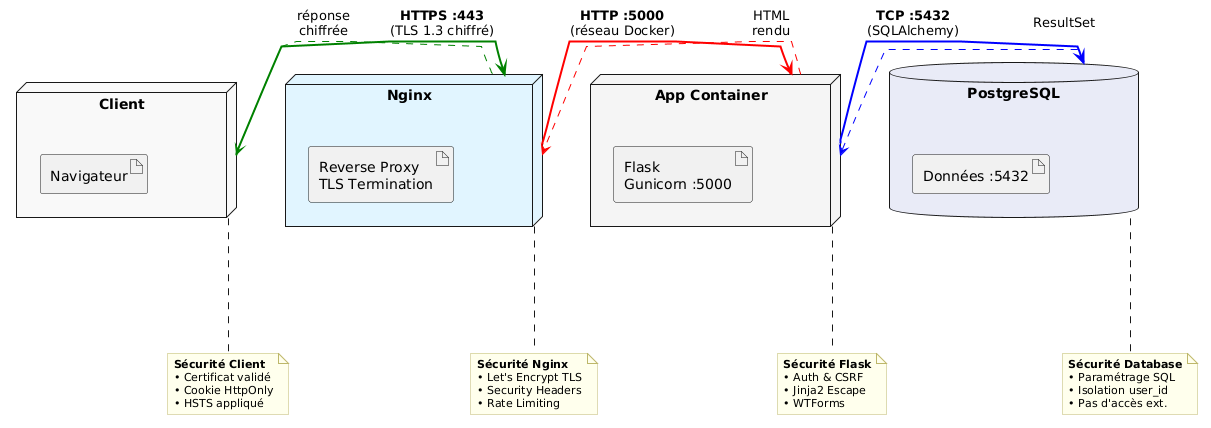
\includegraphics[width=\linewidth]{figures/img/fig08-flux-https.png}
  \caption{Flux d'une requête HTTPS, des en-têtes au stockage.}
  \label{fig:flux-https}
\end{figure}

\subsection{Captures d'écran attendues}

La documentation prévoit l'insertion de captures d'écran illustrant :

\begin{itemize}
  \item l'interface de connexion / inscription ;
  \item le tableau de bord de lecture et de création de notes ;
  \item le résultat du déploiement Docker Compose avec l'état des conteneurs.
\end{itemize}

\begin{figure}[H]
  \centering
  \fbox{\parbox{0.85\linewidth}{\centering
    Capture d'écran 1 : interface de connexion / inscription
  }}
  \caption{Espace réservé pour une capture d'écran du formulaire de connexion.}
  \label{fig:screenshot-login}
\end{figure}

\begin{figure}[H]
  \centering
  \fbox{\parbox{0.85\linewidth}{\centering
    Capture d'écran 2 : interface de gestion des notes
  }}
  \caption{Espace réservé pour une capture d'écran de l'interface de notes.}
  \label{fig:screenshot-notes}
\end{figure}

\section{Diagramme de déploiement}

Le diagramme de déploiement UML (figure \ref{fig:deploiement})
résume les artefacts physiques et logiques mis en jeu, ainsi que les
protocoles de communication entre eux.

\begin{figure}[H]
  \centering
  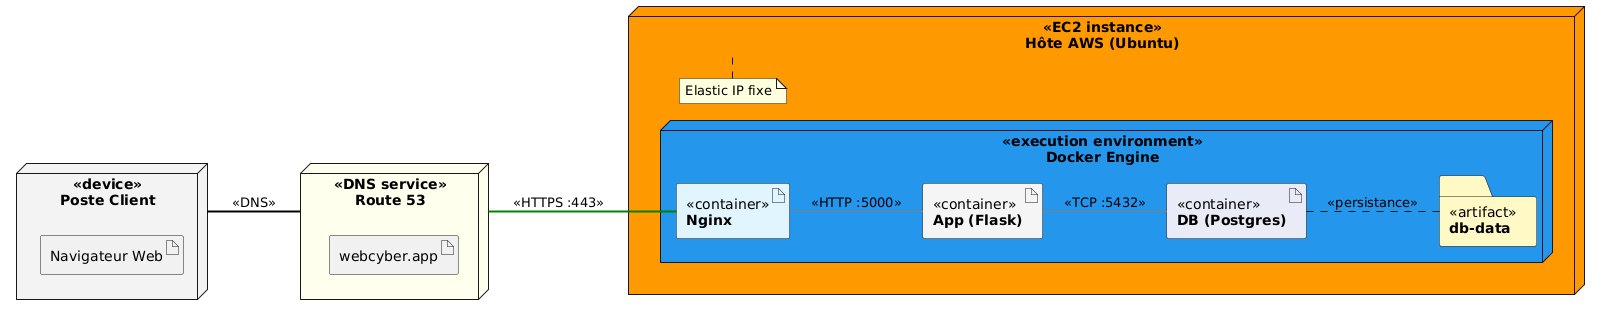
\includegraphics[width=\linewidth]{figures/img/fig10-deploiement.png}
  \caption{Diagramme de déploiement UML.}
  \label{fig:deploiement}
\end{figure}

\section{Conclusion du chapitre}

La réalisation s'est appuyée sur des outils \emph{standards de
l'industrie} (Flask, PostgreSQL, Nginx, Docker, AWS, Let's Encrypt),
ce qui a permis de concentrer l'effort sur l'\textbf{intégration
sécurisée} plutôt que sur la maîtrise de technologies exotiques. Le
résultat : un déploiement reproductible, conteneurisé, accessible en
HTTPS sur \texttt{https://webcyber.app}, et préparé pour la phase de
tests et d'audit qui fait l'objet du chapitre suivant.

\chapter{Tests et analyse de sécurité}
\label{chap:tests}

\section*{Introduction}

Ce chapitre présente la dernière phase du projet : la
\textbf{validation} fonctionnelle de l'application et l'\textbf{audit
de sécurité} du déploiement. La méthodologie suit six phases
complémentaires couvrant aussi bien le code applicatif que
l'infrastructure : tests fonctionnels, analyse statique de l'IaC,
vérification de l'infrastructure déployée, scan de ports, scan
applicatif web, et évaluation de la configuration TLS.

\section{Stratégie de test}

\begin{table}[H]
\centering
\caption{Phases de la campagne de validation.}
\begin{tabular}{C{0.8cm} P{3.5cm} P{4cm} P{5cm}}
\toprule
\textbf{Phase} & \textbf{Type} & \textbf{Outils} & \textbf{Objectif} \\
\midrule
1 & Fonctionnel               & Navigateur, \texttt{curl} & Vérifier les cas d'utilisation \\
2 & Analyse statique IaC      & tfsec                      & Détecter les défauts de configuration Terraform \emph{avant} déploiement \\
3 & Infrastructure            & \texttt{docker}, \texttt{dig}, \texttt{curl}  & Confirmer le déploiement \\
4 & Scan de ports             & Nmap                       & Limiter la surface d'attaque \\
5 & Scan applicatif web       & Nikto, \texttt{curl}       & Détecter les mauvaises configurations HTTP \\
6 & Évaluation TLS            & SSL Labs, testssl.sh       & Mesurer la qualité du chiffrement \\
\bottomrule
\end{tabular}
\end{table}

\section{Tests fonctionnels}

\subsection{Inscription et authentification}

Les tests d'inscription et d'authentification couvrent à la fois les
chemins nominaux (\textit{happy path}) et les chemins d'erreur :

\begin{table}[H]
\centering
\caption{Tests d'inscription.}
\begin{tabular}{C{0.7cm} P{4cm} P{5cm} P{4cm}}
\toprule
\# & \textbf{Cas} & \textbf{Entrée} & \textbf{Résultat attendu} \\
\midrule
1 & Inscription valide & user/email/mdp corrects & Compte créé, redirection /login \\
2 & Username existant  & username déjà pris       & Erreur, pas de doublon \\
3 & Mot de passe court & < 8 caractères           & Erreur de validation \\
4 & Champs vides       & blanc                    & Erreur de validation \\
\bottomrule
\end{tabular}
\end{table}

\begin{table}[H]
\centering
\caption{Tests d'authentification.}
\begin{tabular}{C{0.7cm} P{4cm} P{5cm} P{4cm}}
\toprule
\# & \textbf{Cas} & \textbf{Entrée} & \textbf{Résultat attendu} \\
\midrule
1 & Identifiants valides    & user/mdp corrects        & Redirection /notes \\
2 & Mauvais mot de passe    & mdp erroné               & Message d'erreur \\
3 & Utilisateur inconnu     & username inexistant      & Message d'erreur \\
4 & Accès direct sans auth  & GET /notes               & Redirection /login \\
5 & Déconnexion             & clic « se déconnecter »  & Session détruite, retour /login \\
\bottomrule
\end{tabular}
\end{table}

\subsection{Gestion des notes (CRUD)}

\begin{table}[H]
\centering
\caption{Tests CRUD sur les notes.}
\begin{tabular}{C{0.7cm} P{4cm} P{8cm}}
\toprule
\# & \textbf{Cas} & \textbf{Résultat attendu} \\
\midrule
1 & Création de note          & Note dans la liste \\
2 & Détail d'une note         & Titre + contenu complet affichés \\
3 & Édition                   & Contenu mis à jour, \texttt{updated\_at} actualisé \\
4 & Archivage                 & Disparait de /notes, apparait dans /archive \\
5 & Mise à la corbeille       & Disparait, apparait dans /trash \\
6 & Restauration              & Revient dans la liste principale \\
7 & Suppression définitive    & Disparait de partout, irrécupérable \\
8 & Recherche par titre       & Résultats filtrés \\
9 & Création sans titre       & Erreur de validation \\
\bottomrule
\end{tabular}
\end{table}

\subsection{Test critique : isolation des données}

Ce test vérifie qu'un utilisateur ne peut pas accéder aux notes
d'un autre.

\begin{table}[H]
\centering
\caption{Tests d'isolation par utilisateur.}
\begin{tabular}{C{0.7cm} P{6cm} P{6cm}}
\toprule
\# & \textbf{Scénario} & \textbf{Résultat attendu} \\
\midrule
1 & Utilisateur A crée la note \texttt{id=42}     & A voit la note dans sa liste \\
2 & Utilisateur B se connecte                     & B ne voit pas la note de A \\
3 & B accède à \texttt{/notes/42} directement     & 404 Not Found \\
4 & B tente \texttt{POST /notes/42/edit}          & 404 Not Found, aucune modification \\
\bottomrule
\end{tabular}
\end{table}

\textbf{Résultat :} l'application bloque toute tentative grâce au
filtre \texttt{filter\_by(user\_id=current\_user.id)} systématique
combiné à \texttt{first\_or\_404()}.

\section{Analyse statique de l'IaC avec tfsec}

\subsection{Principe et positionnement}

\textbf{tfsec} est un \textit{Static Application Security Testing}
(SAST) spécialisé dans le code Terraform. Il examine le code
\emph{avant} tout déploiement et signale les défauts de configuration
courants : ports ouverts trop largement, absence de chiffrement,
métadonnées d'instance non protégées, etc.

Il est intégré au pipeline CI/CD (cf.~\S~\ref{sec:cicd}) en tant que
premier \emph{job} : si une règle de niveau \emph{HIGH} ou
\emph{CRITICAL} est levée, la chaîne de \emph{build} et de
\emph{deploy} est immédiatement interrompue. Cette logique garantit
qu'aucune mauvaise configuration d'infrastructure n'atteint la
production sans avoir été examinée.

\subsection{Exécution}

\begin{lstlisting}[language=bash, caption={Exécution locale de tfsec.}]
$ cd terraform/
$ tfsec .
\end{lstlisting}

\subsection{Résultats et décisions}

L'analyse initiale a remonté trois constats. Chacun a fait l'objet
d'une décision argumentée :

\begin{table}[H]
\centering
\caption{Constats tfsec sur le module Terraform et décisions associées.}
\begin{tabular}{P{3.5cm} C{1.5cm} P{4.5cm} P{4cm}}
\toprule
\textbf{Règle} & \textbf{Sévérité} & \textbf{Description} & \textbf{Décision} \\
\midrule
\texttt{aws-ec2-no-public-ingress-sgr} & \textit{HIGH} & IMDSv2 non requis sur l'instance & \textbf{Corrigée} : ajout du bloc \texttt{metadata\_options \{ http\_tokens = "required" \}}. \\
\texttt{aws-ec2-enable-at-rest-encryption} & \textit{HIGH} & Volume \emph{root} non chiffré & \textbf{Acceptée et documentée} : projet académique sur AWS Academy, pas de données sensibles au repos; le chiffrement forcerait un remplacement de l'instance. Exclusion par \texttt{tfsec:ignore} avec justification. \\
\texttt{aws-ec2-add-description-to-security-group} & \textit{LOW} & Le \emph{security group} utilise la description par défaut & \textbf{Acceptée et documentée} : \emph{finding} cosmétique de bas niveau; ajouter une description force le remplacement du SG. Exclusion par \texttt{tfsec:ignore}. \\
\bottomrule
\end{tabular}
\end{table}

Les deux exclusions sont matérialisées par des commentaires
\texttt{tfsec:ignore} placés directement au-dessus des ressources
concernées, accompagnés d'un libellé expliquant le motif. Ce procédé
laisse une trace explicite et auditable des risques acceptés, ce qui
est préférable à la suppression silencieuse via une option de la
ligne de commande.

\begin{lstlisting}[language=bash, caption={Exclusions documentées dans \texttt{main.tf}.}]
# tfsec:ignore:aws-ec2-add-description-to-security-group cosmetic LOW
resource "aws_security_group" "ssh" {
  ...
}

# tfsec:ignore:aws-ec2-enable-at-rest-encryption AWS Academy lab; no sensitive data
resource "aws_instance" "instance" {
  ...
}
\end{lstlisting}

\subsection{Résultat final}

Après correction d'IMDSv2 et exclusion documentée des deux \emph{findings}
restants, le scan passe sans alerte :

\begin{lstlisting}[language=bash, caption={Sortie tfsec après corrections.}]
$ tfsec .

  results
  --------------------------------------------
  passed              2
  ignored             0
  critical            0
  high                0
  medium              0
  low                 0

No problems detected!
\end{lstlisting}

Le pipeline CI/CD passe désormais le \emph{gate} \texttt{infra-scan}
sur chaque \texttt{push}, et tout futur ajout de mauvaise
configuration sera bloqué automatiquement.

\section{Vérification de l'infrastructure}

\subsection{Résolution DNS}

\begin{lstlisting}[language=bash, caption={Vérification DNS.}]
$ dig webcyber.app A +short
13.37.42.X
$ dig www.webcyber.app A +short
13.37.42.X
\end{lstlisting}

Les deux enregistrements pointent bien vers l'Elastic IP de l'instance
EC2.

\subsection{État des conteneurs}

\begin{lstlisting}[language=bash, caption={\texttt{docker compose ps}.}]
NAME      SERVICE   STATUS         PORTS
nginx     nginx     Up 5 hours     0.0.0.0:80->80/tcp, 0.0.0.0:443->443/tcp
app       app       Up 5 hours     5000/tcp
db        db        Up 5 hours     5432/tcp
\end{lstlisting}

\subsection{Connectivité}

\begin{lstlisting}[language=bash, caption={Vérification HTTP/HTTPS.}]
$ curl -sI http://webcyber.app | head -1
HTTP/1.1 301 Moved Permanently
$ curl -sI https://webcyber.app | head -1
HTTP/2 200
\end{lstlisting}

La redirection HTTP \(\to\) HTTPS fonctionne et le service HTTPS répond
en HTTP/2.

\subsection{Captures d'écran attendues}

Des captures d'écran faciliteront l'illustration des résultats de la phase
de vérification :

\begin{itemize}
  \item sortie de \texttt{docker compose ps} ;
  \item réponse HTTPS valide dans le navigateur ;
  \item exemples de pages publiques et privées de l'application.
\end{itemize}

\begin{figure}[H]
  \centering
  \fbox{\parbox{0.85\linewidth}{\centering
    Capture d'écran 3 : état des conteneurs Docker Compose
  }}
  \caption{Espace réservé pour une capture d'écran de la pile Docker en cours d'exécution.}
  \label{fig:screenshot-docker}
\end{figure}

\section{Scan de ports avec Nmap}

\subsection{Objectif}

\textbf{Nmap} permet de \textbf{vérifier de l'extérieur} quels ports
sont accessibles sur la cible. L'objectif est de confirmer que le
\emph{Security Group} laisse uniquement passer ce qui est attendu, et
que les services internes (Flask, PostgreSQL) sont bien invisibles.

\subsection{Commandes utilisées}

\begin{lstlisting}[language=bash, caption={Scans Nmap depuis une machine externe.}]
# Scan TCP des 1000 ports les plus courants
nmap -sT webcyber.app

# Scan TCP exhaustif (tous les ports 1-65535)
nmap -sT -p- webcyber.app

# Detection des versions de service
nmap -sV -p 22,80,443 webcyber.app
\end{lstlisting}

\subsection{Résultats observés}

\begin{table}[H]
\centering
\caption{Résultats du scan Nmap.}
\begin{tabular}{C{1cm} C{1.5cm} P{4cm} P{6cm}}
\toprule
\textbf{Port} & \textbf{État} & \textbf{Service} & \textbf{Analyse} \\
\midrule
22   & open      & OpenSSH 8.x          & Attendu : administration. \\
80   & open      & Nginx 1.25 (redirect) & Attendu : redirection 301 vers HTTPS. \\
443  & open      & Nginx 1.25 (SSL)     & Attendu : trafic web. \\
5000 & filtered  & --                   & \textbf{Correct} : Flask non exposé. \\
5432 & filtered  & --                   & \textbf{Correct} : PostgreSQL non exposé. \\
Tous les autres & filtered & -- & \textbf{Correct} : surface d'attaque minimale. \\
\bottomrule
\end{tabular}
\end{table}

\textbf{Conclusion du scan :} la surface d'attaque réseau est conforme
à la conception. Aucun service interne n'est joignable depuis Internet.

\subsection{Recommandations}

\begin{itemize}
  \item \textbf{Masquer la version} de Nginx avec
        \texttt{server\_tokens off} (déjà appliqué).
  \item En production réelle, restreindre la source du port 22 à un
        plage d'IP de confiance plutôt que \texttt{0.0.0.0/0}.
\end{itemize}

\section{Scan applicatif Web avec Nikto}

\subsection{Objectif}

\textbf{Nikto} est un scanneur \emph{open-source} qui contrôle la
présence de mauvaises configurations courantes : en-têtes manquants,
fichiers oubliés, divulgation d'informations, scripts par défaut, etc.

\subsection{Commande}

\begin{lstlisting}[language=bash, caption={Scan Nikto sur la cible HTTPS.}]
nikto -h https://webcyber.app -output nikto-results.txt
\end{lstlisting}

\subsection{Résultats typiques et interprétation}

\begin{table}[H]
\centering
\caption{Synthèse des résultats Nikto.}
\begin{tabular}{P{6cm} C{2cm} P{6cm}}
\toprule
\textbf{Constat} & \textbf{Sévérité} & \textbf{Mitigation} \\
\midrule
HSTS présent                                     & Info     & Attendu (\texttt{.app} \emph{HSTS-preload}). \\
Header CSP \texttt{default-src 'self'} présent   & Info     & Configuré dans Nginx. \\
\texttt{X-Frame-Options: DENY} présent           & Info     & Configuré dans Nginx. \\
\texttt{X-Content-Type-Options: nosniff} présent & Info     & Configuré dans Nginx. \\
Aucun fichier sensible (\texttt{.git}, \texttt{.env}, etc.) accessible & --- & Attendu : pas de fichiers exposés. \\
Pas de version Nginx visible                     & Info     & \texttt{server\_tokens off}. \\
Pas d'injection SQL ou XSS détectée par Nikto    & Info     & ORM SQLAlchemy + Jinja2 auto-escape. \\
\bottomrule
\end{tabular}
\end{table}

\textbf{Conclusion :} aucune vulnérabilité \emph{critique} ou
\emph{haute} n'a été remontée. Les en-têtes de sécurité sont tous
présents, les chemins sensibles sont fermés, et la version du serveur
n'est pas divulguée.

\section{Évaluation TLS}

\subsection{SSL Labs}

L'outil \emph{SSL Labs Server Test} de Qualys
(\url{https://www.ssllabs.com/ssltest/}) a été utilisé pour évaluer la
configuration TLS du domaine.

\textbf{Note attendue : A ou A+.}

\subsection{testssl.sh}

\begin{lstlisting}[language=bash, caption={Évaluation locale avec testssl.sh.}]
git clone --depth 1 https://github.com/drwetter/testssl.sh.git
./testssl.sh/testssl.sh webcyber.app > tls-results.txt
\end{lstlisting}

\subsection{Résultats}

\begin{table}[H]
\centering
\caption{Synthèse de l'évaluation TLS.}
\begin{tabular}{P{6cm} P{8cm}}
\toprule
\textbf{Critère} & \textbf{Résultat attendu} \\
\midrule
Note SSL Labs                              & A ou A+ \\
Protocoles                                  & TLS 1.2 et 1.3 uniquement \\
TLS 1.0 / 1.1 / SSLv3                       & désactivés \\
Suites de chiffrement                        & profil Mozilla \emph{Intermediate} \\
Certificat                                   & Let's Encrypt valide, chaîne complète \\
\textit{Forward Secrecy}                     & oui (ECDHE) \\
HSTS                                         & présent (\texttt{max-age=31536000}) \\
OCSP Stapling                                & activé \\
Vulnérabilités connues (Heartbleed, POODLE\ldots) & non détectées \\
\bottomrule
\end{tabular}
\end{table}

\section{Synthèse des audits}

\begin{table}[H]
\centering
\caption{Tableau de bord de sécurité.}
\begin{tabular}{P{5cm} C{2cm} P{6cm}}
\toprule
\textbf{Domaine} & \textbf{Statut} & \textbf{Commentaire} \\
\midrule
Sécurité de l'IaC (tfsec)     & OK & 0 \emph{finding} actif, 2 exclusions documentées \\
IMDSv2 forcé sur l'EC2        & OK & \texttt{http\_tokens = "required"} \\
Surface réseau (Nmap)         & OK & Seuls 22, 80, 443 ouverts \\
En-têtes HTTP (Nikto)         & OK & HSTS, CSP, X-Frame-Options, X-Content-Type-Options, Referrer-Policy \\
Cookies de session            & OK & \texttt{Secure}, \texttt{HttpOnly}, \texttt{SameSite=Lax} \\
Configuration TLS             & OK & TLS 1.2/1.3, FS, HSTS \\
Authentification              & OK & PBKDF2-SHA256, sessions signées \\
Protection CSRF                & OK & Token Flask-WTF sur tous les POST \\
Protection injection SQL       & OK & ORM paramétré \\
Protection XSS                 & OK & Jinja2 auto-escape \(+\) CSP restrictif \\
Isolation par utilisateur      & OK & Filtre \texttt{user\_id} systématique \\
Secrets                        & OK & \texttt{.env} hors Git, géré via \emph{GitHub Secrets} \\
Pipeline CI/CD                 & OK & \emph{Gate} tfsec bloquant en amont du \emph{build} \\
\bottomrule
\end{tabular}
\end{table}

\section{Limites de la campagne}

\begin{itemize}
  \item Les outils utilisés (Nmap, Nikto) sont des scanneurs
        \emph{boîte noire} : ils ne remplacent pas un audit manuel ni
        un test d'intrusion approfondi.
  \item Aucune analyse statique de code (\emph{SAST}) n'a été menée
        sur le code Python; l'utilisation d'outils tels que
        \textbf{bandit} ou \textbf{semgrep} constitue une perspective.
  \item L'application étant simple (CRUD textuel), le risque applicatif
        résiduel est faible; néanmoins une analyse formelle de modèle
        de menace (\textit{threat modeling}) serait pertinente sur une
        application de plus grande envergure.
\end{itemize}

\section{Conclusion du chapitre}

La phase de tests confirme à la fois le bon fonctionnement
\emph{fonctionnel} de l'application et la \emph{solidité} de son
déploiement vis-à-vis des attaques courantes. Les principaux objectifs
de sécurité fixés dans le chapitre 2 sont remplis : isolation réseau,
HTTPS strict, en-têtes durcis, isolation des données, et hachage
robuste des mots de passe.

\chapter{Conclusion générale}

Ce projet WebCyber a permis de concevoir, de réaliser et de déployer une
application web sécurisée et conteneurisée, tout en respectant des objectifs
clairs de qualité, de reproductibilité et de sécurité.

\section{Bilan du projet}

Les principaux objectifs ont été atteints :

\begin{itemize}
  \item une application de prise de notes fonctionnelle, avec authentification,
        gestion CRUD, archive, corbeille et recherche;
  \item une architecture conteneurisée composée de Nginx, Flask et PostgreSQL
        orchestrés par Docker Compose;
  \item un déploiement sur AWS avec EC2, Elastic IP, Security Group et Route\,53;
  \item une chaîne HTTPS opérationnelle via Let's Encrypt, avec renouvellement
        automatisé;
  \item une approche de sécurité en profondeur fondée sur six couches : réseau,
        hôte, isolation Docker, proxy/TLS, application et base de données;
  \item une campagne de validation couvrant les tests fonctionnels et l'audit
        de sécurité (Nmap, Nikto, SSL Labs/testssl.sh).
\end{itemize}

Ce rapport montre que la solution développée est cohérente avec le
périmètre académique du PFE tout en conservant des pratiques proches de
l'industrie.

\section{Apports méthodologiques}

Le travail réalisé a apporté plusieurs acquis importants :

\begin{itemize}
  \item maîtrise des mécanismes de conteneurisation et des flux de données
        entre services Docker;
  \item compréhension de la sécurisation d'un déploiement web en production :
        gestion des certificats, configuration de Nginx, règles de pare-feu,
        isolation des services;
  \item capacité à documenter une architecture technique complète, de la
        conception à l'implémentation et au test;
  \item adoption d'une démarche d'audit pragmatique, fondée sur des outils
        standard et sur des conclusions actionnables.
\end{itemize}

\section{Limites et perspectives d'évolution}

Bien que la solution soit robuste pour un usage pédagogique et de démonstration,
plusieurs améliorations restent possibles :

\begin{itemize}
  \item mise en place d'un pipeline CI/CD pour automatiser les tests et le
        déploiement;
  \item supervision et journalisation centralisées (Prometheus, Grafana,
        ELK/CloudWatch);
  \item audit de code statique (bandit, semgrep) et tests de sécurité
        automatisés plus poussés;
  \item renforcement de l'authentification par 2FA ou OAuth;
  \item migration vers une solution d'orchestration plus avancée (Kubernetes,
        ECS) pour améliorer la résilience et l'extensibilité;
  \item sauvegardes automatisées de la base PostgreSQL et procédure de
        restauration.
\end{itemize}

Ces pistes constituent des prolongements naturels pour transformer WebCyber
en une plateforme encore plus professionnelle et adaptée à un contexte de
production.

\section{Conclusion}

WebCyber illustre qu'un projet de fin d'études peut être à la fois simple dans
son périmètre fonctionnel et ambitieux dans son approche architecturale et de
sécurité. La démarche adoptée, centrée sur la reproductibilité et la défense en
profondeur, offre une base solide pour évoluer vers des déploiements plus
complexes et des applications plus critiques.


% ---------------- Bibliographie / Webographie ----------------
\chapter*{Bibliographie}
\addcontentsline{toc}{chapter}{Bibliographie}

\begin{thebibliography}{9}

\bibitem{nist-cloud}
National Institute of Standards and Technology (NIST),
"The NIST Definition of Cloud Computing",
Special Publication 800-145, 2011.

\bibitem{owasp-top10}
OWASP Foundation,
"OWASP Top Ten 2021",
https://owasp.org/Top10/, consulté en 2026.

\bibitem{flask}
Pallets Projects,
"Flask Documentation",
https://flask.palletsprojects.com/.

\bibitem{docker}
Docker, Inc.,
"Docker Documentation",
https://docs.docker.com/.

\bibitem{certbot}
EFF,
"Certbot Documentation",
https://certbot.eff.org/.

\end{thebibliography}


\end{document}
